\section{Neintegrální charakteristiky}
\begin{define}
	Mějme $ X\sim f_X$. Potom definujeme \textbf{módy} $f_X$ jako $\{x ~|~ f_X(x)\text{ má v }x\text{ max} \}$.
\end{define}
\begin{remark}
	Unimodální rozdělení je takové rozdělení, které má pouze jedno maximum.
\end{remark}
\begin{define}
	X má \textbf{symetrické rozdělení okolo 0}, pokud $X\sim \PP^X \Leftrightarrow -X\sim \PP^X$. \newline
	X má \textbf{symetrické rozdělení okolo $a$}, pokud $X-a$ má symetrické rozdělení okolo 0.
\end{define}
\begin{remark}
	Chyták ke zkoušce: na Lebesgueově míře toto platí, ale obecně nemusí.
\end{remark}
\begin{define}
	$X\sim \FF_X(=\PP^X/\tau_1)$. Definujeme \textbf{$\alpha$-kvantil rozdělení} $\FF_X$ jako \newline $x_\alpha=\inf\{ x:\FF_X(x)\geq \alpha \}$ pro $\forall \alpha \in [0,1]$.
\end{define}
\begin{define}
	Nechť $X\sim \PP^X(\FF_X)$ a $\alpha\in(0,1)$. Potom $\alpha$-kvantil $x_\alpha = \inf\{ x:\FF_X(x)\geq \alpha \}$. Definujeme následující výrazy:
	\begin{enumerate}
		\item $x_{1/2}$ - \textbf{medián} ($X\sim f_X$ ASR)
		\item $x_{1/4} ~a~ x_{3/4}$ - \textbf{kvartily}
		\item $(x_{3/4}-x_{1/4})$ - \textbf{interkvartilové rozpětí}
		\item $x_{\alpha~100\%}$ - \textbf{percentil}
	\end{enumerate}
\end{define}
\begin{figure}[h]
	\centering
	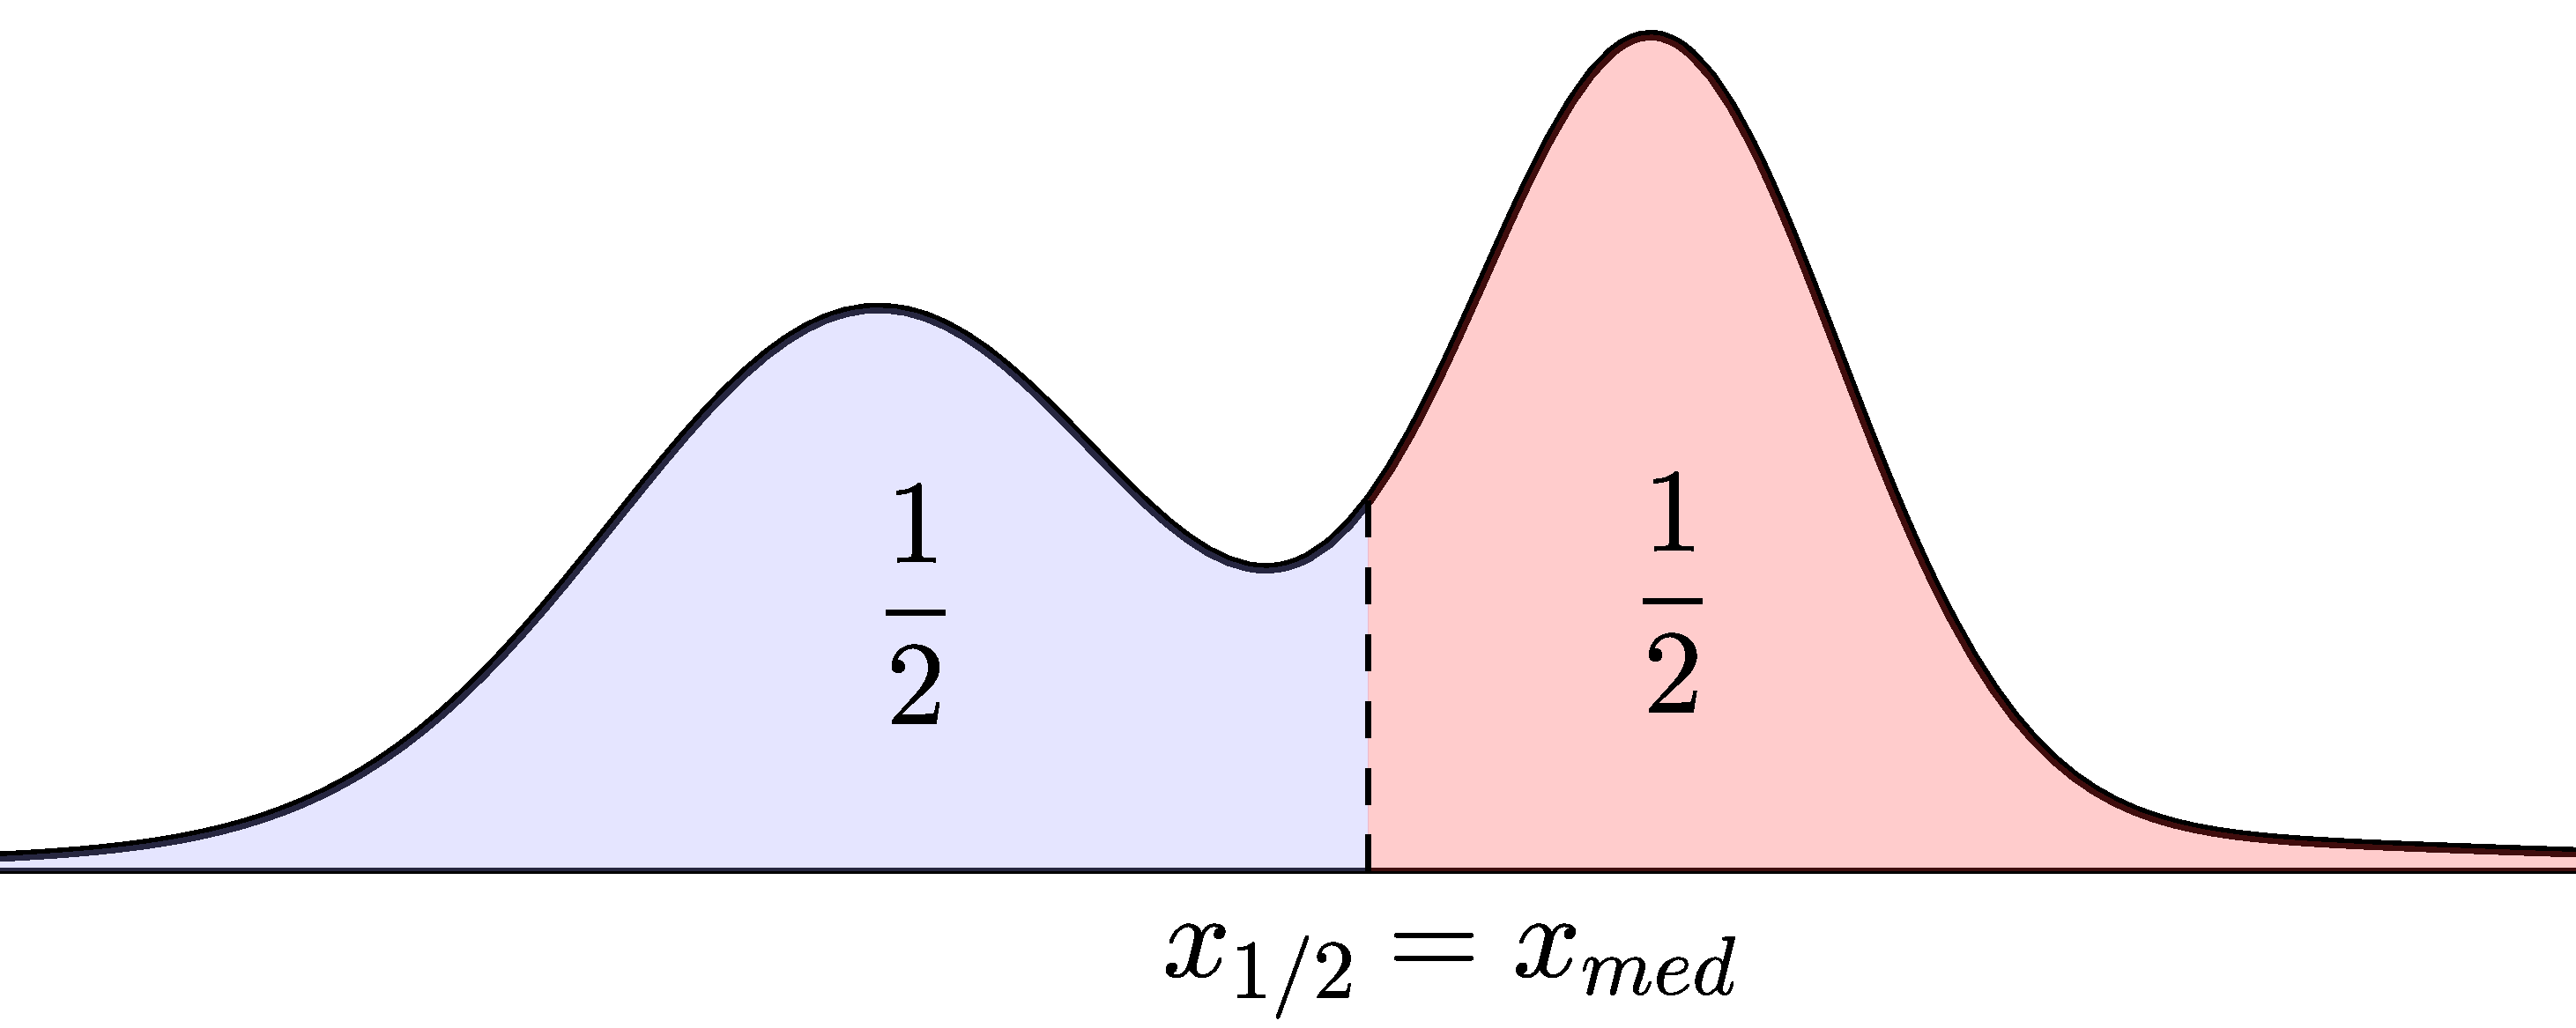
\includegraphics[width=0.4\linewidth]{median}
	\hspace{0.5cm}
	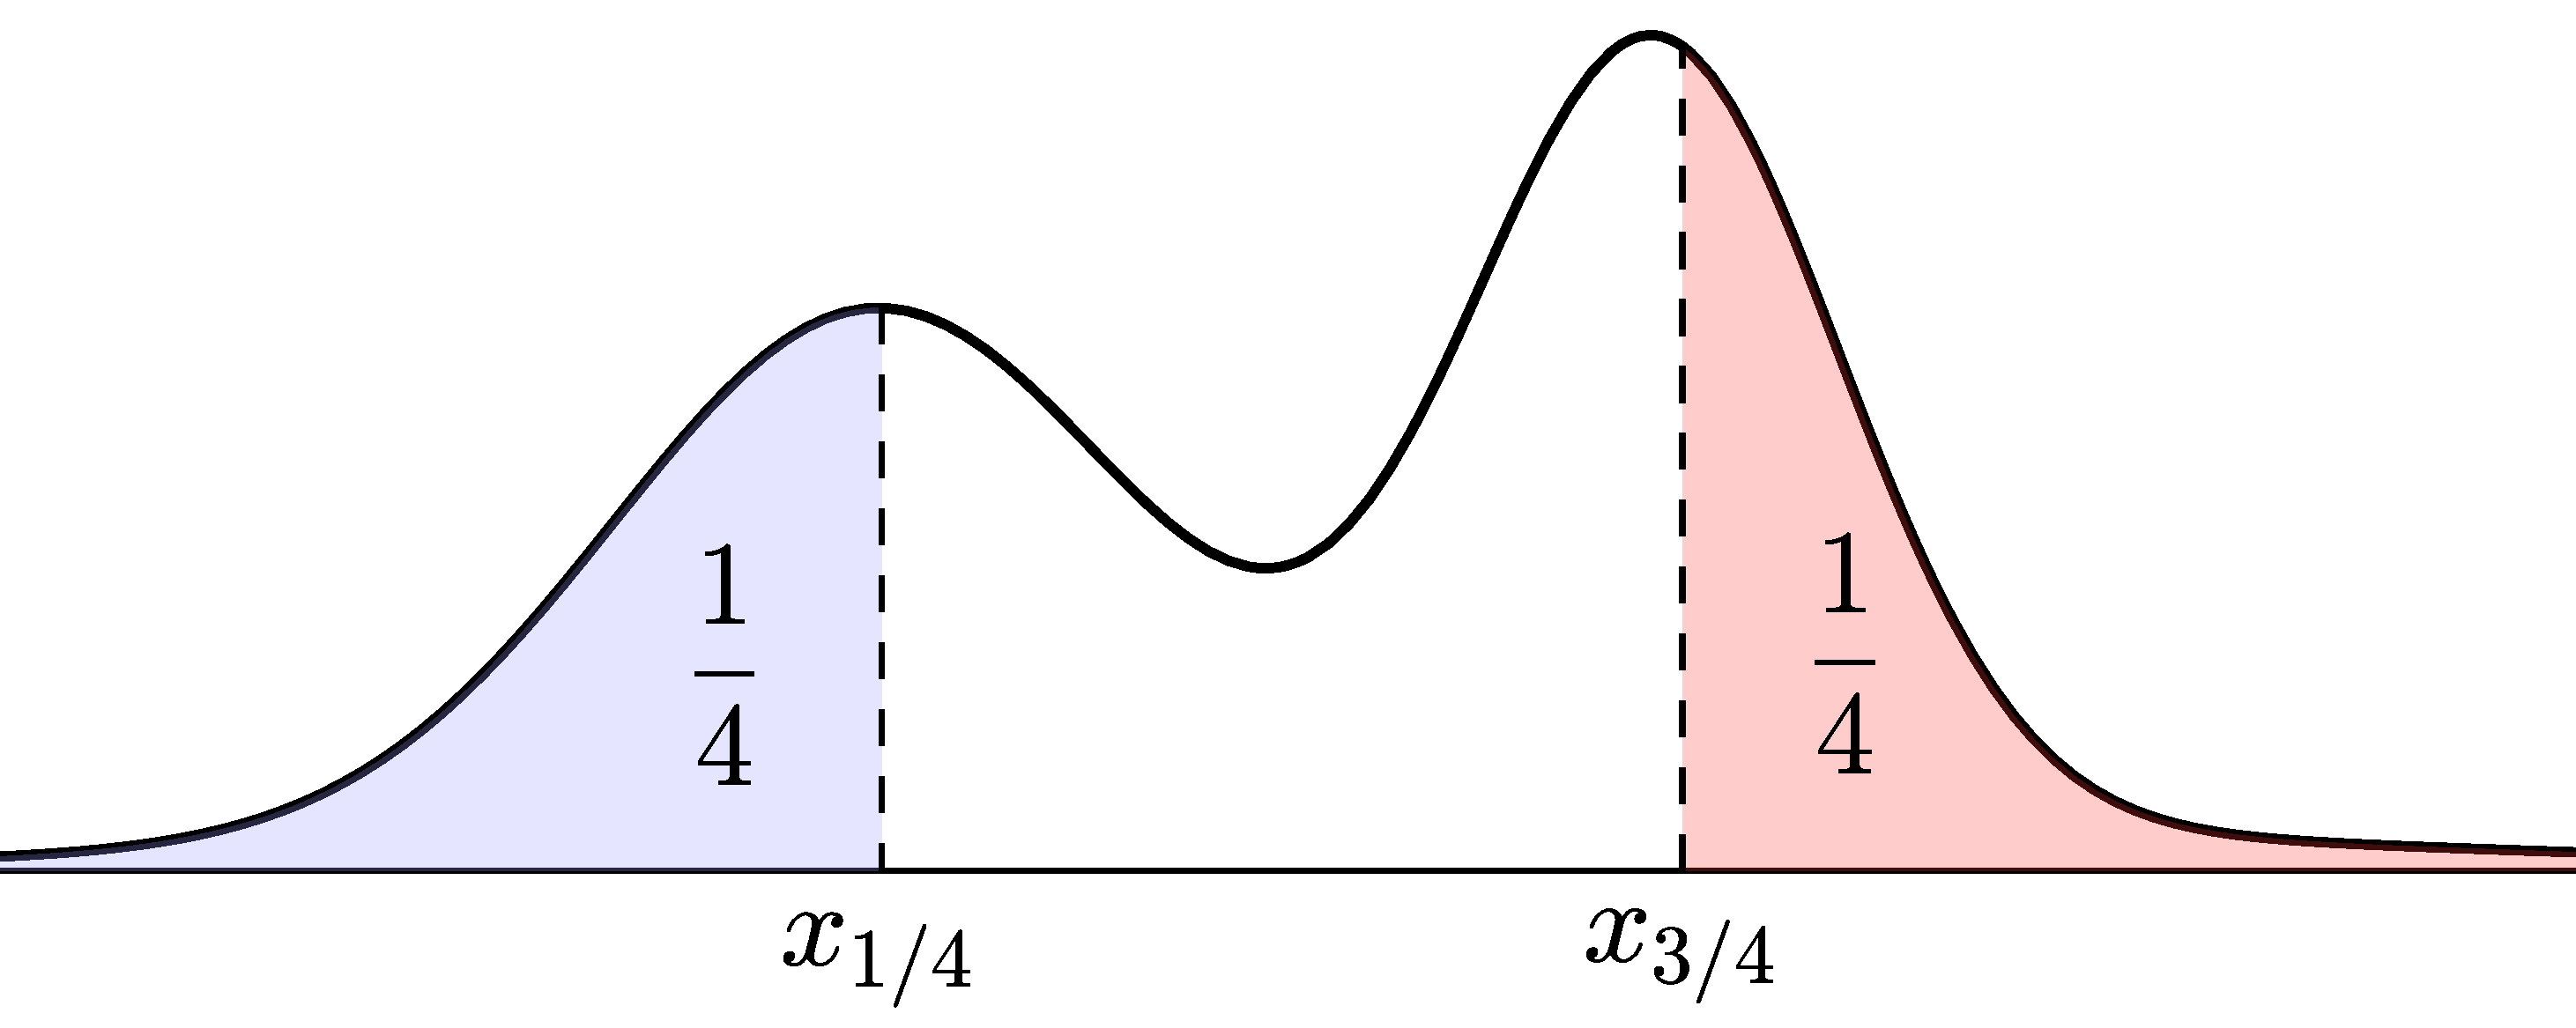
\includegraphics[width=0.4\linewidth]{kvartily}
	\caption{Medián (vlevo) a kvartily (vpravo)}
	\label{fig:median}
\end{figure}

\begin{example}
	\begin{enumerate}
		\item $\alpha=0 ~\Rightarrow~ x_0=-\infty$
		\item \[\alpha=1 ~\Rightarrow~ x_1=\inf\{ x:\FF_X(x)\geq 1 \}=\begin{cases}
		\inf \emptyset=+\infty \\
		x_F~(\text{pravý kraj})<+\infty
		\end{cases}
		\]
	\end{enumerate}
\end{example}
\begin{figure}[h]
	\centering
	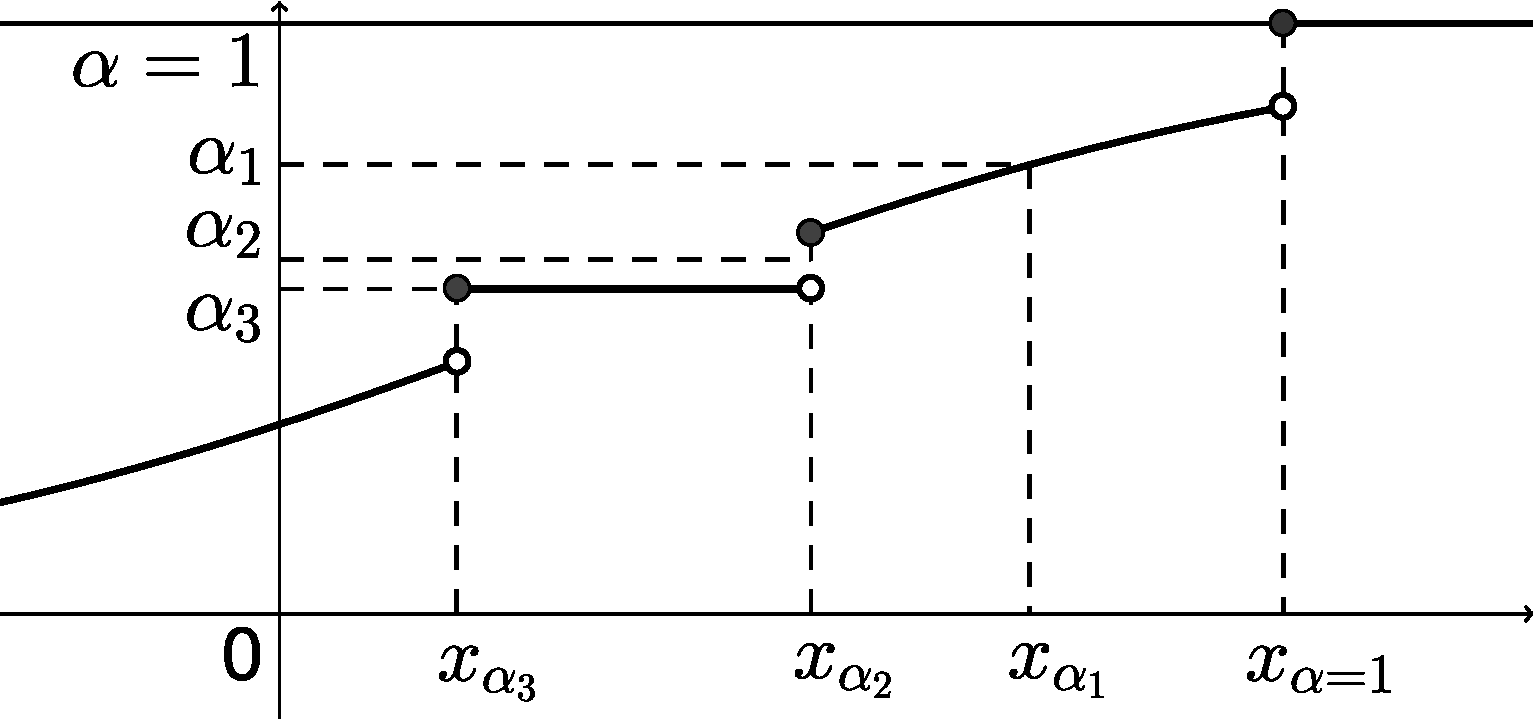
\includegraphics[width=0.60\linewidth]{neintegralnicharakteristiky1}
	\label{fig:neintegralnicharakteristiky1}
\end{figure}

\begin{theorem}
	Nechť $X\sim \FF_X$ je symetrická okolo $a\in\R$ a ostře roste. Pak\newline $x_\alpha = 2a-x_{1-\alpha}~~\forall \alpha\in(0,1)$. Speciálně pro $a=0$ tedy platí, že $x_\alpha = -x_{1-\alpha}$. (obr. \ref{fig:symetrie})
	\begin{proof}
		$\FF_X$ je spojitá $~\Rightarrow~\bigl(\forall \alpha\in(0,1)\bigr)\bigl(x_\alpha=\FF_X^{-1}(\alpha)\bigr)$
		\[
		\begin{split}
		\alpha&=\FF_X(x_\alpha)=\PP(X\leq x_\alpha)=\PP(X-a\leq x_\alpha-a)\equal{\text{sym.}}\PP(-X+a\leq x_\alpha-a)=\PP(X\geq 2a-x_\alpha)= \\ &=1-\PP(X< 2a-x_\alpha)\equal{\text{spoj.}}1-\PP(X\leq 2a-x_\alpha)=1-\FF_X(2a-x_\alpha)
		\end{split}
		\] 
	\end{proof}
\end{theorem}
\begin{figure}[h]
	\centering
	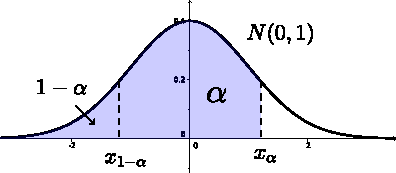
\includegraphics[width=0.4\linewidth]{symetrie}
	\caption{Symetrické rozdělení okolo 0.}
	\label{fig:symetrie}
\end{figure}
\begin{remark}~
		\begin{itemize}
		\item $N(\mu,\sigma^2)$ je symetrický okolo $\mu$
		\item $t(n)$ je symetrický okolo 0 ~~~$[t_\alpha(n)=-t_{1-\alpha}(n)]$
		\item Cauchy$(0,1)$ je symetrický okolo 0 ~~~$[c_\alpha=-c_{1-\alpha}]$
		\item 	$$ X\sim F(n,m)\equal{\text{i.d.}}\frac{\chi^2(n)/n}{\chi^2(m)/m}\Leftrightarrow \frac{1}{X}\sim F(m,n)$$ $$[F_\alpha(n,m)=\frac{1}{F_{1-\alpha}(m,n)}]  \stackrel{DCv}{~\Longrightarrow~} 2a-x_\alpha=x_{1-\alpha} $$
	\end{itemize} 

\end{remark}
\begin{define}
	Mějme $X\sim \FF_X$. Pro $\forall t \in(0,1)$ je definována \textbf{kvantilová funkce} jako $$ \FF_X^\leftarrow(t):=\inf\{ x:\FF_X(x)\geq t \}, $$ ozn. také $\FF_X^-$ nebo $\FF_X^{-1}$ (zobecněná inverzní funkce).
\end{define}
\begin{remark}
	Čtenář může rozmyslet, jestli \begin{enumerate}
		\item když $\FF_X$ je spojitá a ostře roste, pak $\FF_X^\leftarrow=\FF_X^{-1}$ jako inverzní funkce.
		\item když $\FF_X$ ostře roste, pak $\FF_X^\leftarrow=\FF_X^{-1}$ na $\dom{\FF_X^{-1}} $.
	\end{enumerate}
\end{remark}
\section{Integrální charakteristiky}
\begin{define}
	Mějme $\prostor$ a $\lambda$ $\sigma$-finitní. Pak funkci $\lphi(\omega):=\sum\limits_{j=1}^k a_j \mathbb{I}_{A_j}(\omega)$, kde\newline $\forall j\in\hat{k},~A_j\in\mathcal{A},~a_j\in\R$, nazýváme \textbf{simple function} (jednoduchá funkce). Definujeme dále
	\begin{enumerate}
		\item 
		$$ \int\limits_{\Omega} \lphi \dif \PP_\lambda :=\sum\limits_{j=1}^k a_j \PP(A_j). $$
		\item $X\geq 0$ je náhodná veličina. Pak definujeme $\int\limits_\Omega X\dif \PP=\sup\{ \int\limits_\Omega \lphi \dif \PP: \lphi\text{ simple},~0\leq \lphi\leq X \}$ \newline $[\exists \lphi_n\geq 0,\lphi_n \to X~~a~~\int\limits_{\Omega}X\dif \PP=\lim\limits_{n\to+\infty}\int\limits_{\Omega}\lphi_n\dif \PP_\lambda]$
		\item $X$ je libovolná náhodná veličina. Pak definujeme $\int\limits_{\Omega}X\dif \PP=\int\limits_{\Omega}X^+ \dif \PP-\int\limits_{\Omega}X^-\dif \PP$ za předpokladu konečnosti alespoň jednoho integrálu. Označme dále$$\E X=\int\limits_{\Omega}X\dif \PP=\int\limits_{\Omega}X(\omega )\dif \PP(\omega)=\int\limits_{\Omega}X\PP(\dif\omega)$$ jako \textbf{střední hodnotu}. (angl. \textbf{expected value}).
		\item Pro $\mathbb{X}:\Omega\to\R^n$ jako náhodnou veličinu definujeme $\E \mathbb{X}=(\E X_1,...,\E X_n)$.
		\item $A\in\mathcal{A}$ definujeme $\int\limits_{A}X\dif \PP=\int\limits_{\Omega}X \mathbb{I}_A\dif \PP$, speciálně pro $X\equiv 1$ pak $$\int\limits_{A}1\dif \PP_\lambda = \PP_\lambda(A)=\int\limits_{\Omega}\mathbb{I}_A\dif \PP_\lambda=\E (\mathbb{I}_A)$$
	\end{enumerate}
\end{define}	
\begin{remark}
	Symbol $\Omega$ pod integrálem se často vynechává.
\end{remark}
\begin{define}
	Označme $\LL_1=\{ X\text{ n.vel. na }\prostor: |\E X|<+\infty \}=\LL_1\prostor$.
\end{define}
\begin{theorem}
	$\LL_1$ je vektorový prostor a $\E $ je lineární funkcionál na $\LL_1$, "tzn." $$\E \Bigl( \sum\limits_{j=1}^n \alpha_jX_j \Bigr)=\sum\limits_{j=1}^n \alpha_j \E X_j.$$
\end{theorem}
\begin{theorem}
	$X\in\LL_1 \Leftrightarrow |X|\in\LL_1$ ~~~a~~~ $|\E X|\leq \E |X|$.
	\begin{proof}
		Viz MAA/MAB.
	\end{proof}
\end{theorem}
\begin{dusl}
	$\LL_1\prostor~\Rightarrow~$ každá omezená náhodná veličina je integrovatelná.\begin{proof}
		$$ |\E X|\leq \E |X|\leq \E K=K\E (1)=K\int\limits_{\Omega}1\dif \PP=K \PP(\Omega)=K, $$ kde $K$ je konstanta.
	\end{proof}
\end{dusl}
\begin{theorem}
	Mějme $X,Y$ náhodné veličiny na $\prostor$ tak, že $\E X,~\E Y$ existují a nechť $\PP(\underbrace{X=Y}_{A})=1$. Pak $\E X=\E Y$.
	\begin{proof}
		$$\E (X-Y)=\int\limits_{\Omega}(X-Y)\dif \PP=\int\limits_{A\in\mathcal{A}}(X-Y)\dif \PP+\int\limits_{A^c}(X-Y)\dif \PP=0+0=0$$
	\end{proof}
\end{theorem}
\begin{define}
	$\prostor$. Pak $N\subset \Omega$ se nazývá \textbf{nulová množina} (pro $\PP$), pokud $\exists A\in\Aa$, $N\subset A$ a platí, že $\PP(A)=0$. Definujme nyní 
	$$ \Nn= \{ N \subset \Omega: N\text{ je nulová vzhledem k }\PP \}. $$ Potom řekneme, že nějaká vlastnost V platí \textbf{skoro jistě na $\PP$} ($s.j.~\PP$), pokud $\exists N\in\Nn$ tak, že tato vlastnost V platí na $\Omega \setminus N.$ 
\end{define}
\begin{remark}
	Někdy se také značí $a.s.~\PP$ (almost sure) nebo w.r.t. $\PP$ (with respect to).
\end{remark}
\begin{define}
	$\prostor$. Definujeme $\bar{\Aa}=\Aa\cup\Nn :=\{ A\cup N:A\in\Aa,N\in\Nn \}$ jako \textbf{zúplnění} $\sigma$-algebry $\Aa$. \newline Definujeme dále $\bar{\PP}$ tak, že $\bar{\PP}(A\cup N)=\PP(A),~~\forall A\in\Aa,\forall N\in\Nn$ jako \textbf{rozšíření} $\PP$ z $\Aa$ na $\bar{\Aa}$.\newline
	$\prostor$ $\to (\Omega,\bar{\Aa},\bar{\PP})$: 
	$$ A=\emptyset\in\Aa ~\Rightarrow~ \bar{\PP}(N)=\bar{\PP}(A\cup N)=\bar{\PP}(\emptyset\cup N)=\PP(\emptyset)=0,~~\forall N\in\Nn $$
\end{define}
\begin{remark}
	Tvrdíme, že $\bar{\PP}$ je pravděpodobnostní míra na $(\Omega,\bar{\mathcal{A}})$ a je jednoznačná.
	\begin{proof}
		Jednoznačnost $\bar{\PP}$: volme $C\in\bar{\Aa}$, předpokládejme, že  $C=A_1\cup N_1=A_2\cup N_2\subset A_2\cup B_2$, kde $  N_2\subset B_2$ a $\PP(B_2)=0$ (analogicky pak zavedeme $B_1$). Potom platí, že 
		\[
		\begin{split}
		\bar{\PP}(A_1\cup N_1)&=\PP(A_1)\leq \PP(A_2\cup B_2)\leq \PP(A_2)+\PP(B_2)=\bar{\PP}(A_2\cup N_2)=\PP(A_2)\leq\\ &\leq \PP(A_1\cup B_1)\leq  \PP(A_1)+\PP(B_1)=\bar{\PP}(A_1\cup N_1) 
		\end{split}
		\] 
		Z toho vyplývá, že $ \bar{\PP}(A_1\cup N_1)=\bar{\PP}(A_2\cup N_2) $. Nyní ověříme, že se jedná o pravděpodobnost.
		\begin{enumerate}
			\item $\bar{\PP}(\Omega)=\bar{\PP}(\Omega\cup \emptyset)=\PP(\Omega)=1$
			\item $\bar{\PP}(C)\geq 0,~~~\forall C\in\Aa$
			\item \[
			\begin{split}
			\bar{\PP}\Bigl( \underbrace{\sum\limits_{n=1}^{+\infty}}_{disj.}\underbrace{C_n}_{\in\bar{\Aa}} \Bigr)&=\bar{\PP}\left(\sum\limits_{n=1}^{+\infty} (A_n\cup N_n)\right)=\bar{\PP}\Bigl( \underbrace{\sum\limits_{n=1}^{+\infty} A_n}_{\in\Aa}\cup \underbrace{\sum\limits_{n=1}^{+\infty} N_n}_{\in\mathcal{N}} \Bigr)=\PP\Bigl( \sum\limits_{n=1}^{+\infty} A_n \Bigr)= \\ &=\sum\limits_{n=1}^{+\infty} \PP(A_n) =\sum\limits_{n=1}^{+\infty} \bar{\PP}(A_n\cup N_n)=\sum\limits_{n=1}^{+\infty} \bar{\PP}(C_n)
			\end{split}
			\] 
		\end{enumerate}
	\end{proof}
\end{remark}

\begin{theorem}
	Mějme X,Y tak, že $\E X$, $\E Y$ existuje a nechť $X=Y$ $s.j.~\PP$. Pak $\E X=\E Y$.
\end{theorem}
\begin{remark}
	Domluva: $\bar{\Aa}$ ozn. $\Aa$, $\bar{\PP}$ ozn. $\PP$.
\end{remark}
\begin{define}
	$X=Y~ s.j.~\PP$ je relací ekvivalence $X\sim Y$. Vezměme nyní $\LL_1$ a definujme $\L_1\prostor:=\LL_1 /_\sim$. Pro $T\in \L_1$ (T je třída ekvivalence) definujeme $\E (T)=\E (X)$, kde $X\in T$. Dále definujeme na $\L_1$ \textbf{normu} $\left\|X\right\|_{\L_1}:=\E |X|$. $($na $\LL_1$ je to pseudonorma$)$
\end{define}
\begin{remark}
	Bývá zvykem místo $s.j.~\PP$ psát pouze $s.j.$\newline Relace ekvivalence obecně znamená, že "předefinujeme" rovnítko jiným vztahem, např. $s.v.$ nebo $s.j.~P$. V tomto případě je tedy $T\in \L_1$ "balíček" všech $X_n$, kde pro $\forall i,j$ platí, že $X_i=X_j$ $s.j.~\PP$.
\end{remark}
\begin{remark}
	$\left\|X\right\|_{\L_1}=0\Leftrightarrow X=0$. Na $\LL_1$ však $\left\|X\right\|_{\L_1}=0\Leftrightarrow X=0$ $s.j.~\PP$.
\end{remark}
\begin{define}
	$\L_1\prostor$ je lineární normovaný prostor s normou $\left\|~\right\|_{\L_1}$. Říkáme, že\newline $X_n\stackrel{\L_1}{\to}X$, pokud $\left\|X_n-X\right\|_{\L_1}\to 0$. ($\L_1$ je Banachův prostor)
\end{define}
\begin{theorem}~
	\begin{enumerate}[a)]
		\item 	$X\leq Y$ s.j. $~\Rightarrow~ \E X\leq \E Y$ (za předpokladu existence).
		\item $X\geq 0$ $s.j.~\PP~\Rightarrow~ \E X\geq 0$
	\end{enumerate}
\end{theorem}
\begin{figure}[h]
	\centering
	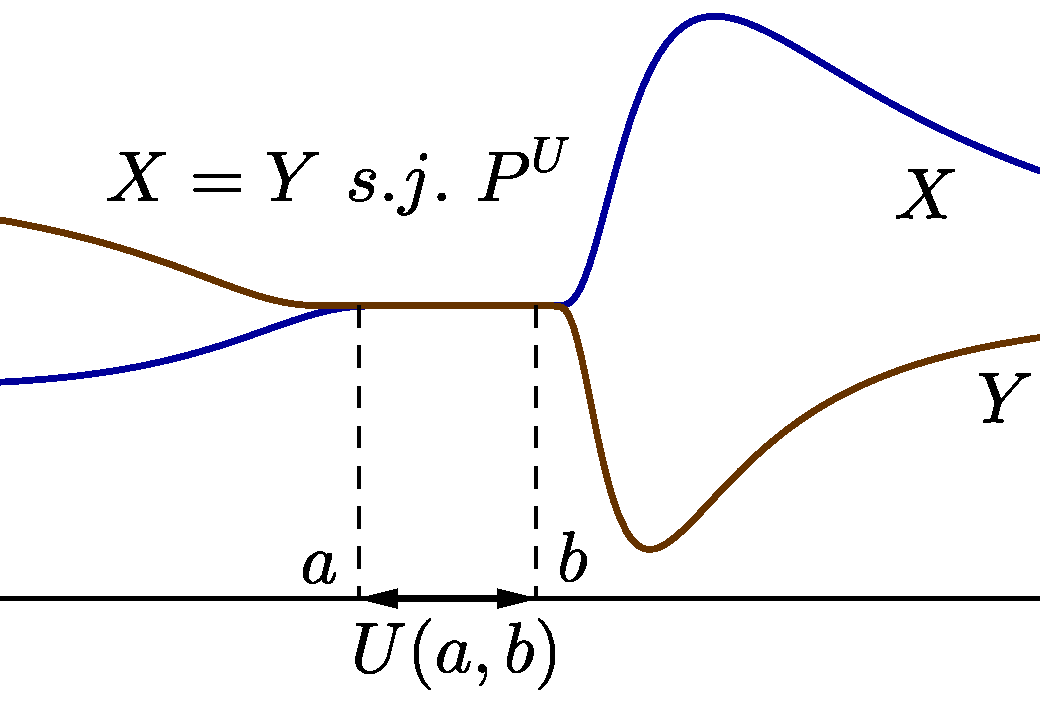
\includegraphics[height=3cm]{sj1}
	\hspace{0.4cm}
	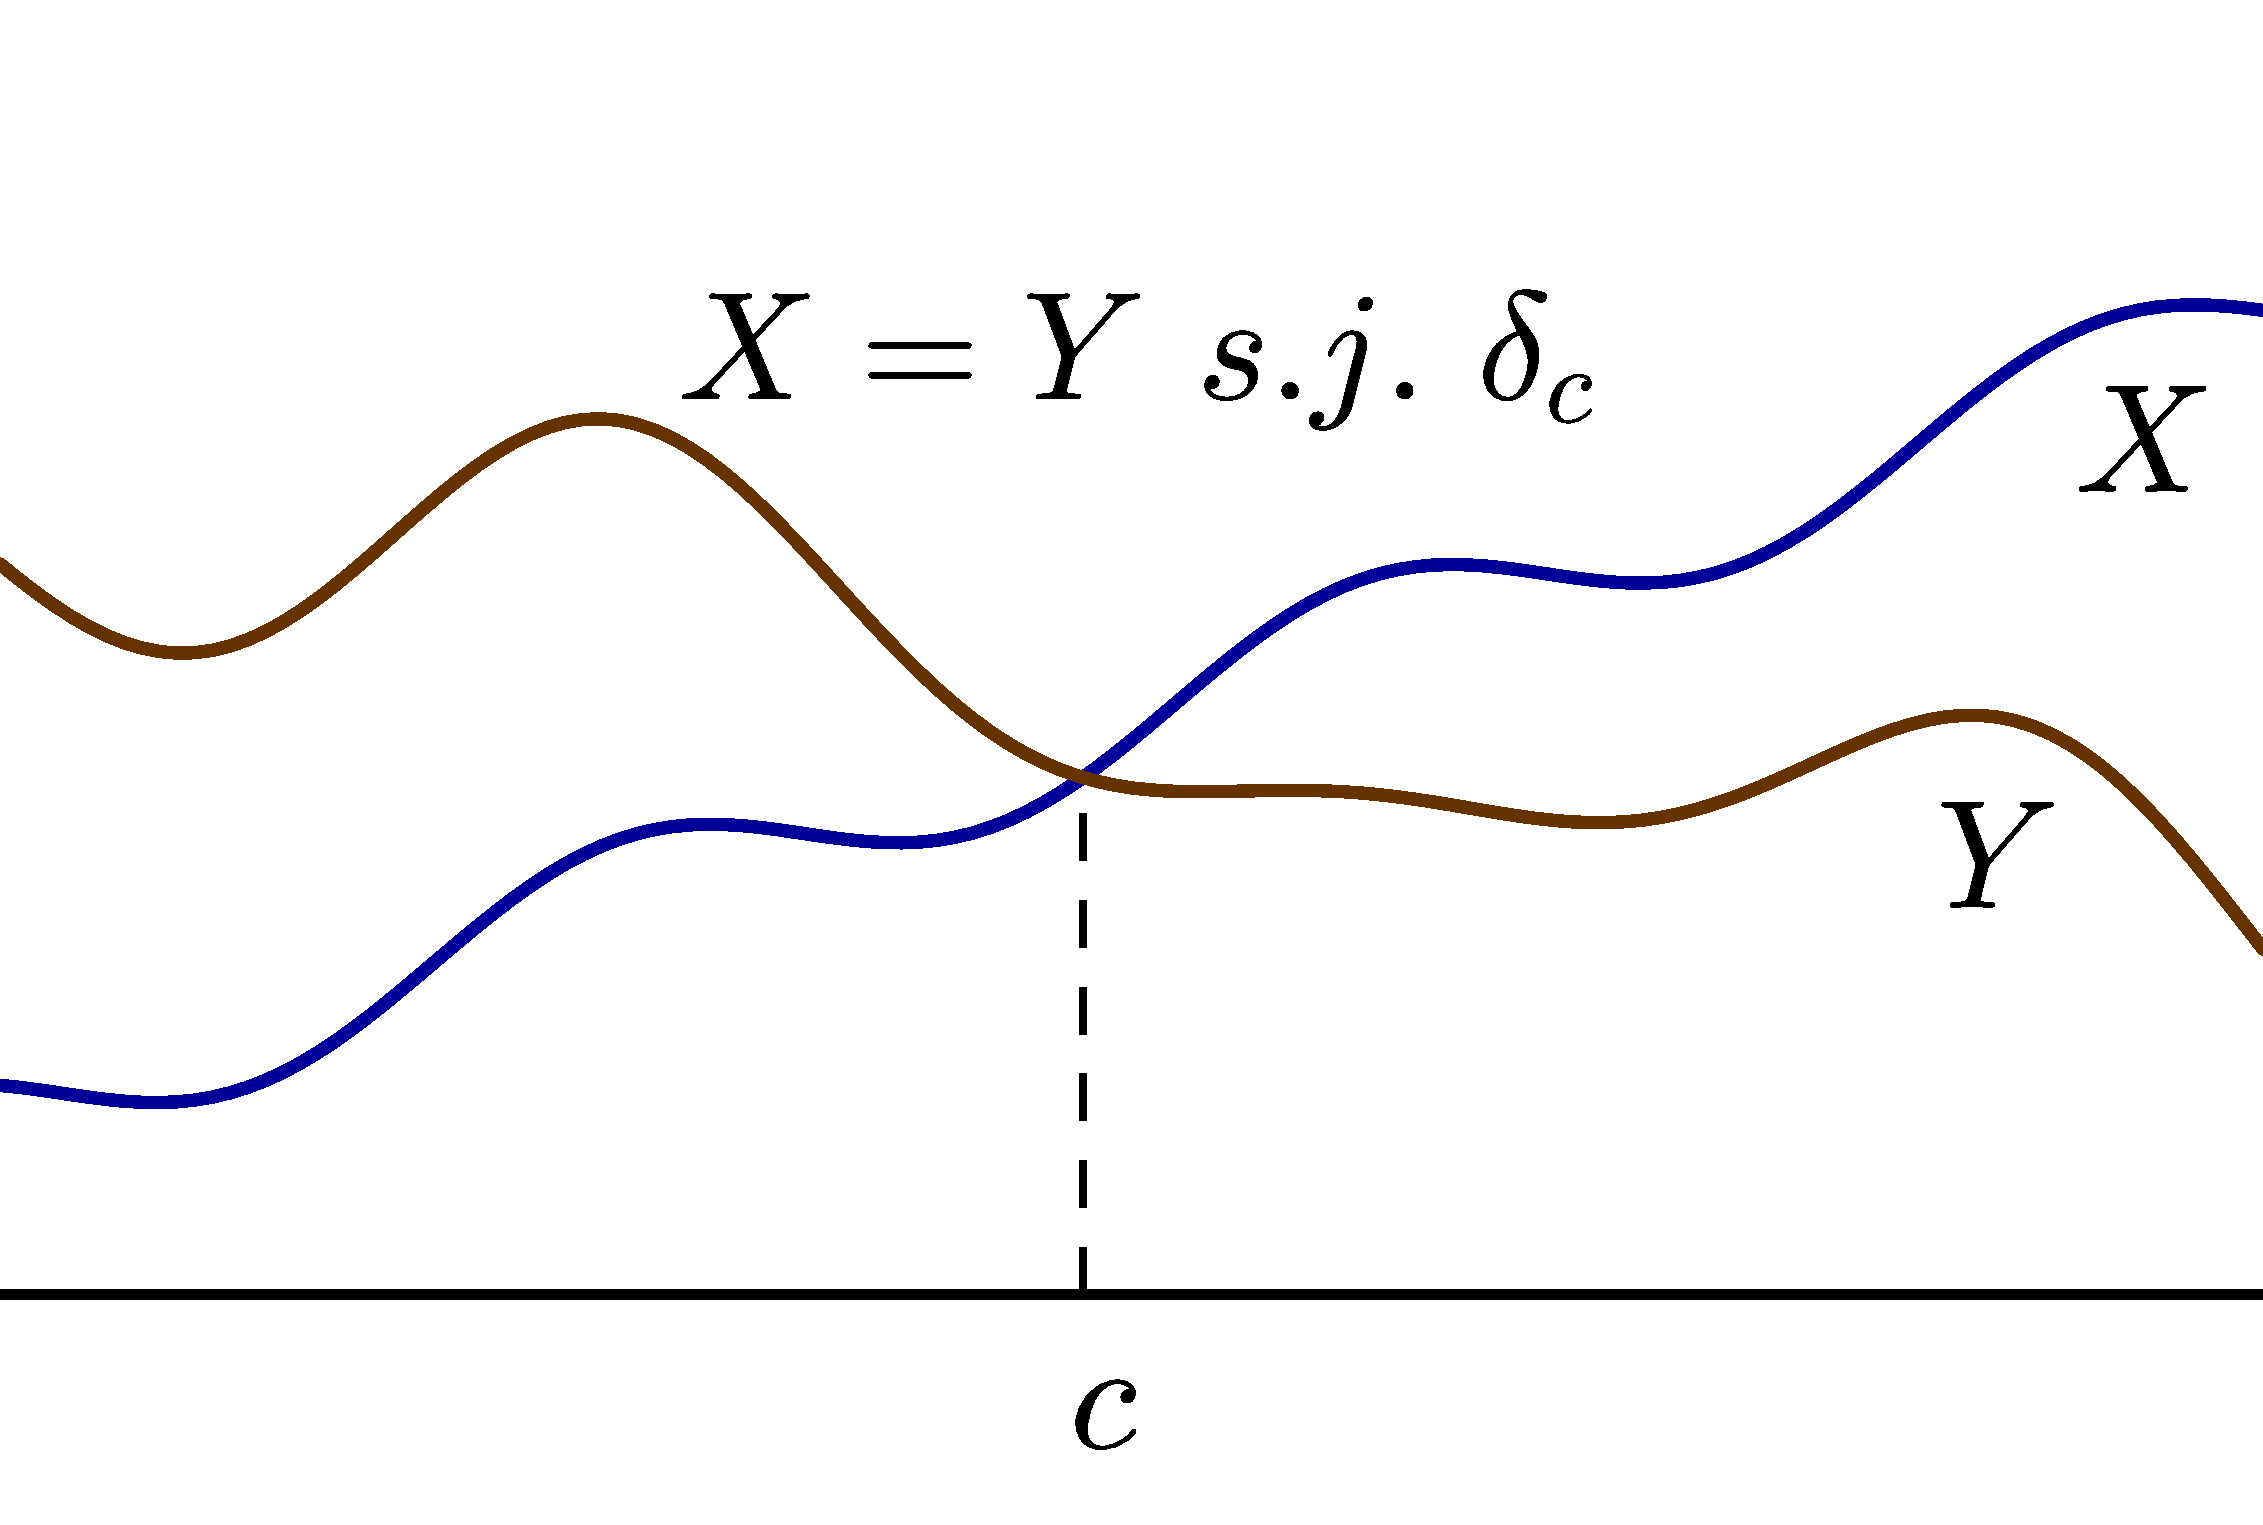
\includegraphics[height=3cm]{sj2}
	\hspace{0.4cm}
	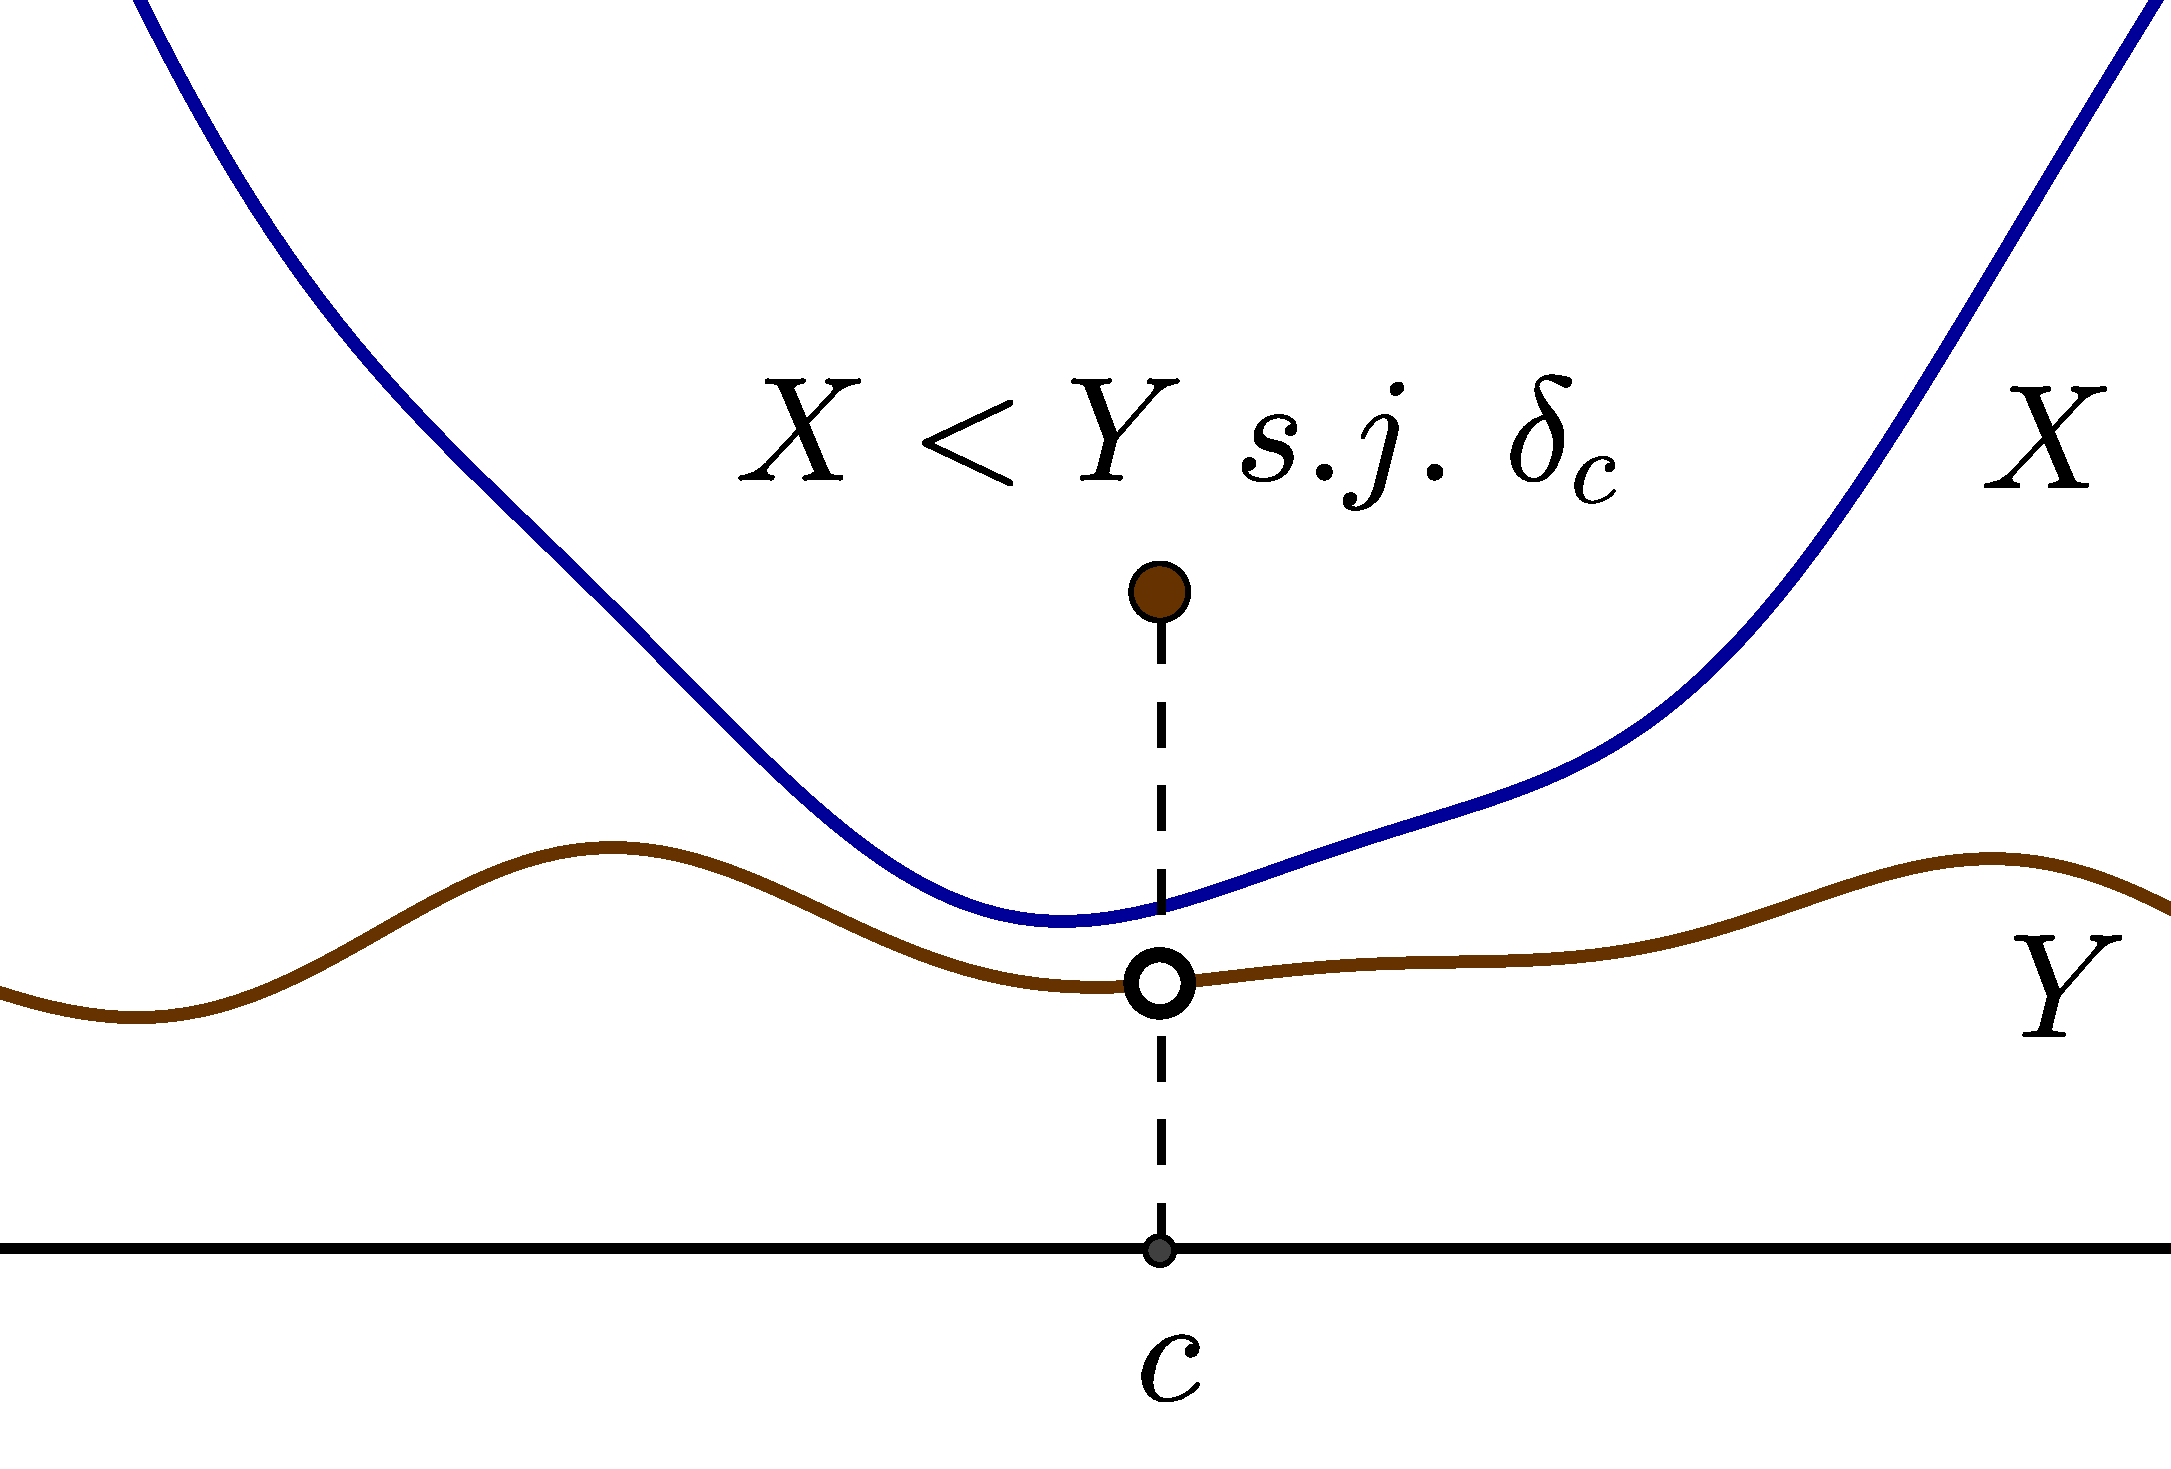
\includegraphics[height=3cm]{sj3}
	\label{fig:sj1}
\end{figure}

\begin{theorem}[MCT - Monotone Convergence Theorem]
	Mějme $(\Omega,\Aa,\PP_\lambda)$, $X_n\geq 0$ $s.j.~\PP$ a $X_n \nearrow X$ $s.j.~\PP$. Pak $\E X_n \to \E X$.
\end{theorem}
\begin{theorem}[LDCT - Lebesgue's Dominated Convergence Theorem]
	Mějme $(\Omega,\Aa,\PP_\lambda)$,\newline $X_n\to X$ $s.j.~\PP$ a $|X_n|\leq Y$ $s.j.~\PP$, kde $Y\in\LL_1$. Pak $X_n\in\LL_1,~X\in\LL_1$ a $\E X_n\to \E X$.
\end{theorem}
\begin{theorem}[Beppo-Levi]
		Nechť $\posln$ jsou náhodné veličiny na $\prostor$ tak, že\newline $\sum\limits_{n=1}^{+\infty} \underbrace{\E |X_n|}_{\left\|X_n\right\|_{\L_1}}<+\infty$. Pak $\sum\limits_{n=1}^{+\infty} X_n<+\infty$ $s.j.~\PP$, $\underbrace{\sum\limits_{n=1}^{+\infty} X_n}_Y\in\LL_1$ a $\E \left( \sum\limits_{n=1}^{+\infty} X_n \right)=\sum\limits_{n=1}^{+\infty} \E X_n$.
		\begin{proof}
			$$ \left| \sum\limits_{j=1}^n X_j \right|\leq \sum\limits_{j=1}^n |X_j|\leq \sum\limits_{j=1}^{+\infty} |X_j|\equal{\text{ozn.}}S,~~~\forall n\in\N $$
			$$ \E S=\E \underbrace{\left( \sum\limits_{j=1}^{+\infty} |X_j| \right)}_{\sum\limits_{j=1}^{n}|X_j|\nearrow S}=\sum\limits_{j=1}^{+\infty} \E |X_j|<+\infty~\Rightarrow~ S<+\infty \text{ s.j.} $$
			$$\int\limits_{\Omega}S\dif \PP<+\infty~\Rightarrow~ S<+\infty \text{ s.j.} $$
			Sporem: $S=+\infty$ s.j., tzn. $\PP(\{ \omega:S(\omega)=+\infty \})>0 ~\Rightarrow~ \int\limits_{\Omega}S\dif \PP=+\infty$
			$$ \E \left( \sum\limits_{j=1}^{+\infty} X_j \right)=\E \left( \lim\limits_{ n\to +\infty}\sum\limits_{j=1}^n X_j \right)\equal{\text{LDCT}}\lim\limits_{ n\to +\infty} \E \left( \sum\limits_{j=1}^n X_j \right)=\lim\limits_{ n\to +\infty}  \sum\limits_{j=1}^n \E X_j=\sum\limits_{j=1}^{+\infty} \E X_j $$
		\end{proof}
	\end{theorem}
\begin{theorem}[Markovova nerovnost]
	Mějme $X\in\LL_1$ na $\prostor$. Pak $(\forall\epsilon>0)\left(\PP(|X|\geq\epsilon)\leq \frac{\E |X|}{\epsilon}\right)$.
	\begin{proof}
	$$ \E |X|\geq \E [|X|\cdot \mathbb{I}_{\{ |X|\geq\epsilon \}}]\geq \E [\epsilon\cdot \mathbb{I}_{\{|X|\geq\epsilon\}}]=\epsilon \E [\mathbb{I}_{\{|X|\geq\epsilon\}}]=\epsilon\int\limits_{\Omega}\mathbb{I}_{\{|X|\geq\epsilon\}}\dif \PP=\epsilon\int\limits_{\{|X|\geq\epsilon\}}1\dif \PP=\epsilon \PP(|X|\geq\epsilon) $$
	\end{proof}
\end{theorem}
\begin{theorem}[Jensensenova nerovnost]
	Mějme $X\in\LL_1$, $\Phi:\R\to\R$ konvexní na intervalu $\I$ tak, že $\PP(X\in \I)=\PP^X(\I)=1$. Pokud $\Phi(X)\in\LL_1$, pak $\E [\Phi(X)]\geq \Phi(\E X)$.\begin{proof}
		Nechť $L$ je tečna funkce $\Phi$ v bodě $\E X$.\newline
			\begin{tabular}{m{8cm} m{8cm}}
			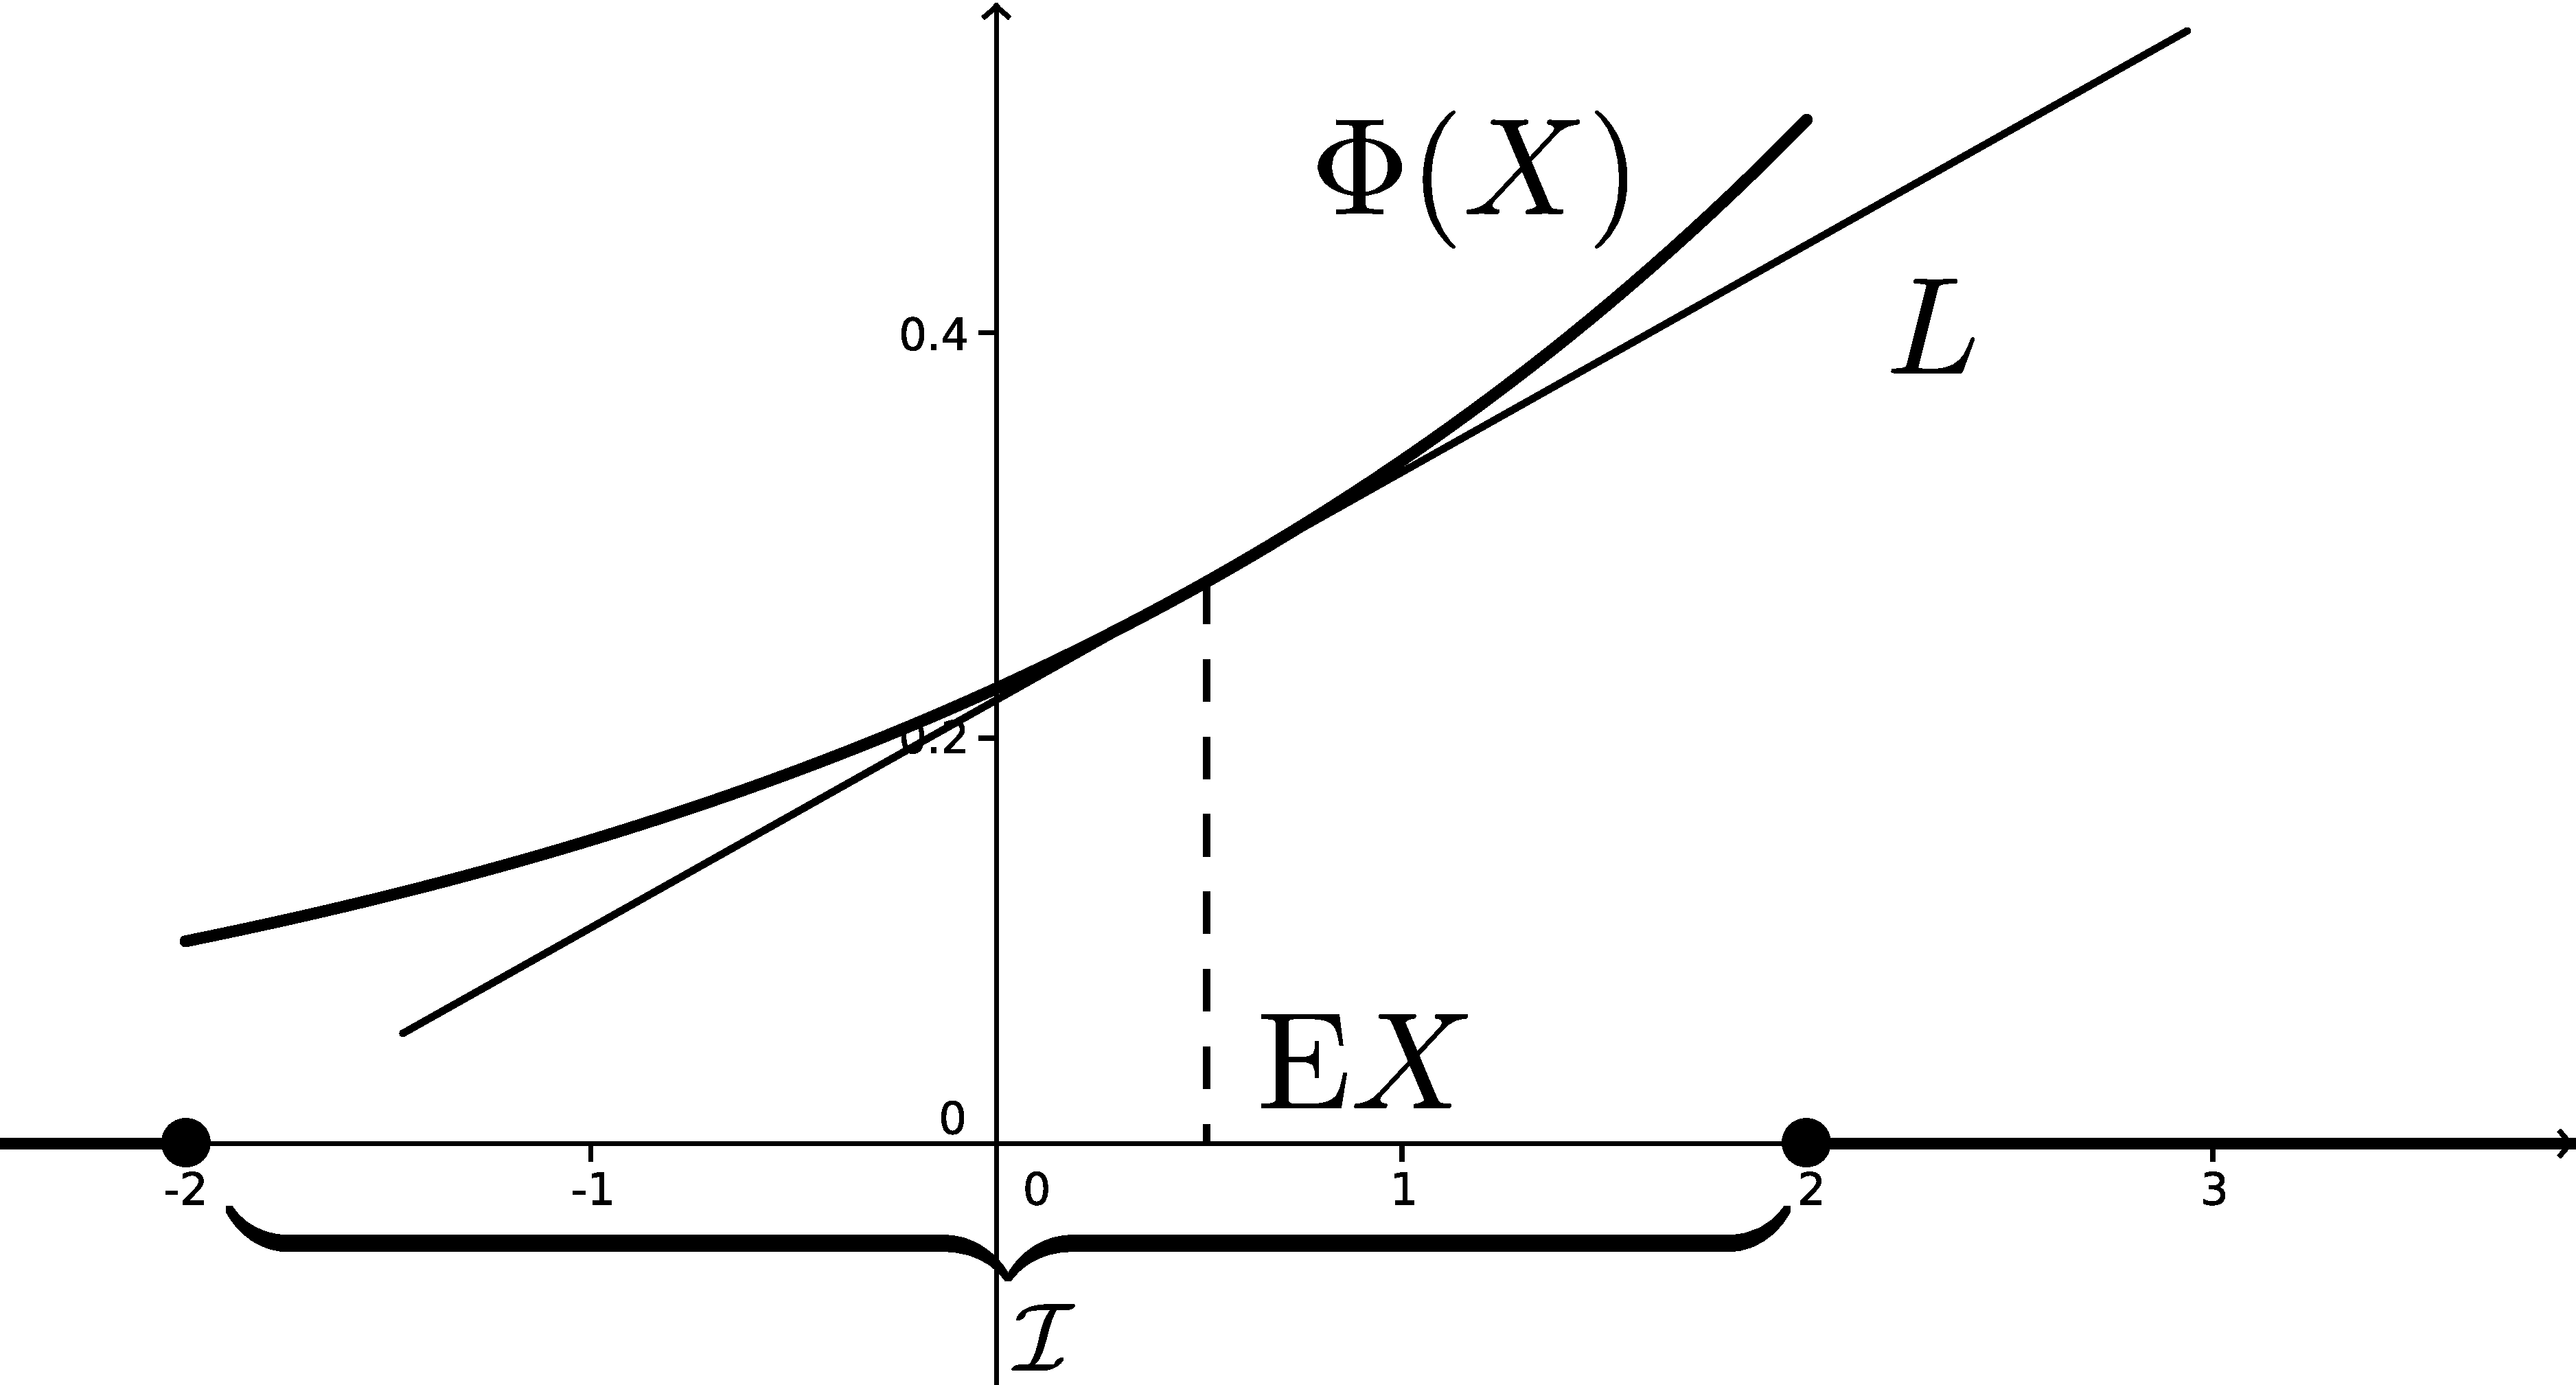
\includegraphics[width=8cm]{tecna} & $ \E [\Phi(X)]\geq \E [L(X)]=L(\E X)=\Phi(\E X)$ 
			\end{tabular} 
	\end{proof}
\end{theorem}

\begin{dusl}
	$\Phi(t)=t^2~\Rightarrow~ \E (X^2)\geq (\E X)^2$
\end{dusl}
\begin{define}
	Mějme $(\Omega_j,\Aa_j,\PP_j)~\forall j\in\hat{n}$. Definujme $\bigtimes\limits_{j=1}^n \Aa_j:=\{ \bigtimes\limits_{j=1}^n A_j:A_j\in\Aa_j \}$. Dále pak definujeme $\bigotimes\limits_{j=1}^n \Aa_j=\sigma(\bigtimes\limits_{j=1}^n \Aa_j)$ a $\bigotimes\limits_{j=1}^n \PP_j$ předpisem pro její funkční hodnoty na generujícím systému $\bigtimes\limits_{j=1}^n \Aa_j$ jako 
	$$ \bigotimes\limits_{j=1}^n \PP_j\Bigl(\bigtimes\limits_{j=1}^n A_j\Bigr)=\prod\limits_{j=1}^n \PP_j(A_j),~\forall A_j\in\Aa_j $$ a nazýváme ji \textbf{součinová míra}.
\end{define}
\begin{theorem}
	Součinová míra existuje, je jednoznačná a je to pravděpodobnostní míra.
\begin{proof}
	korektnost pro n=2: $ C\in\bigotimes\limits_{j=1}^2 \Aa_j $ a definujeme $(\PP_1\bigotimes \PP_2)(C):=\int\limits_{\Omega_1}\PP_2(C(\omega_1))\dif \PP_1$, kde 	\begin{tabular}{p{10cm} m{6cm}}
	$C(\omega_1)=\{ \omega_2:(\omega_1,\omega_2)\in C \}$ je řez C pro fixní $\omega_1$. & 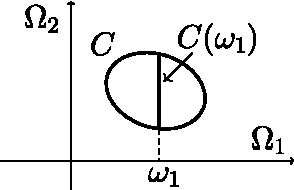
\includegraphics[width=4cm]{C}
	\end{tabular} 
	\begin{enumerate}[a)]
		\item pokud $C=A_1\times A_2,~A_1\in\Aa_1,~A_2\in\Aa_2$, tak
		\[
		\PP_1\bigotimes \PP_2(C)= \int\limits_{A_1}\PP_2(A_2)\dif \PP_1=\PP_2(A_2)\int\limits_{A_1}\dif \PP_1=\PP_1(A_1)\PP_2(A_2),~\text{ protože }C(\omega_1)=\begin{cases}
		A_2 & \forall \omega_1\in\Aa_1 \\ \emptyset & \text{jinde}
		\end{cases}
		\]
		\item $\PP_1 \bigotimes \PP_2$ je pravděpodobnost:\begin{enumerate}[1)]
			\item $(\PP_1\bigotimes \PP_2)(\Omega_1 \times \Omega_2)=\PP_1(\Omega_1)\PP_2(\Omega_2)=1$
			\item $\PP_1\bigotimes \PP_2 \geq 0$
			\item $\sigma$-aditivita: pro $(C_k)_{k=1}^{+\infty}\in\Aa_1\bigotimes\Aa_2$: \[
			\begin{split}
			\PP_1\bigotimes \PP_2\left(\sum\limits_{k=1}^{+\infty} C_k\right)&=\int\limits_{\Omega_1}\PP_2\left(\Bigl( \sum\limits_{k=1}^{+\infty} C_k \Bigr)(\omega_1)\right)\dif \PP_1=\int\limits_{\Omega_1}\PP_2\left( \sum\limits_{k=1}^{+\infty} C_k(\omega_1) \right)\dif \PP_1= \\ &=\int\limits_{\Omega_1}\sum\limits_{k=1}^{+\infty} \underbrace{\PP_2(C_k(\omega_1))}_{\geq 0}\dif \PP_1\equal{\text{MCT}}\sum\limits_{k=1}^{+\infty} \int\limits_{\Omega_1}\PP_2(C_k(\omega_1))\dif \PP_1=\sum\limits_{k=1}^{+\infty} \PP_1\bigotimes \PP_2(C_k)
			\end{split}\]\end{enumerate}
			\item jednoznačnost: $\PP_1\bigotimes \PP_2$ je pravděpodobnost na $\Aa_1\bigotimes \Aa_2$ definovaná na $\Aa_1\times\Aa_2$ předpisem $\PP_1\bigotimes \PP_2=\prod\limits_{j=1}^2 \PP_j(A_j)$, přičemž $\Aa_1\times\Aa_2$ generuje $\Aa_1\bigotimes\Aa_2$ a $\Aa_1\times\Aa_2$ je uzavřený na konečné průniky. Tvrzení pak vyplývá z věty o jednoznačnosti rozšíření.
		
	\end{enumerate}
\end{proof}
\end{theorem}
\begin{theorem}
	Mějme $(X_j)_{j=1}^n$ náhodné veličiny na $\prostor$ a $\X\sim \PP^\X$. Pak $(X_j)_{j=1}^n$ jsou nezávislé $\Leftrightarrow \PEX = \bigotimes\limits_{j=1}^n \PP^{X_j}$.\begin{proof}
		$(X_j)_{j=1}^n$ jsou nezávislé $\stackrel{\text{def}}{\Longleftrightarrow}\underbrace{\PP(X_1\in\Bb_1,...,X_n\in\Bb_n)}_{=\PP(\X\in\bigtimes\limits_{j=1}^n B_j)=\PEX(\bigtimes\limits_{j=1}^n B_j)}=\underbrace{\prod\limits_{j=1}^n \PP(X_j\in\Bb_j)}_{=\prod\limits_{j=1}^n \PP^{X_j}(B_j)}~~~\forall B_j\in\Bb$
		$$ ~\Rightarrow~ \PEX \text{ splňuje definici podmínky ze součinové míry, tzn. }\PEX=\bigotimes\limits_{j=1}^n \PP^{X_j}\text{ (z jednoznačnosti)} $$
	\end{proof}
\end{theorem}
\begin{remark}
	Náhodné veličiny $\posl$ jsou nezávislé $\Leftrightarrow(\forall n\in\N)(\PEX=\bigotimes\limits_{j=1}^n \PP^{X_j}). $
\end{remark}
\begin{theorem}[Tonelli-Fubini]
	Mějme $(\Omega_1,\Aa_1,\PP_1),(\Omega_2,\Aa_2,\PP_2)$ a nechť $X:\Omega_1\times\Omega_2\to\R$ je náhodnou veličinou na $(\Omega_1\times\Omega_2,\Aa_1\bigotimes\Aa_2)$. Pak
	$$\E ^{\PP_1\bigotimes \PP_2}(X)=\E ^{\PP_2}\left[ \E ^{\PP_1}(X) \right]\text{ za předpokladu existence }\E ^{\PP_1\bigotimes \PP_2}(X).$$
\end{theorem}
\begin{remark}
	$\int\limits_{\Omega_1\times\Omega_2}X\dif(\PP_1\bigotimes \PP_2):=\int\limits_{\Omega_2}\left(\int\limits_{\Omega_1}X\dif \PP_1\right)\dif \PP_2$. 
	Fubini lze použít pouze na\newline prostoru se součinovou mírou.
\end{remark}
\begin{remark}
	Speciálně pokud $(\R,\Bb,\lambda_1)(\R,\Bb,\lambda_2);f(x,y):\to\R$ měřitelná, pak $$\int\limits_{\R\times\R}f\underbrace{\dif\lambda^{(2)}}_{\dif x\dif y}=\int\limits_{\R}\int\limits_{\R}f\underbrace{\dif\lambda_1}_{\dif x}\underbrace{\dif\lambda_2}_{\dif y}.$$
\end{remark}
\begin{theorem}
	Nechť $X\geq 0$ je jednorozměrná náhodná veličina na $\prostor$. Pak $$\E X=\int\limits_{0}^{+\infty}(1-\FF_X(x))\dif x.$$\begin{proof}
		\[
		\begin{split}
		&\int\limits_{0}^{+\infty}(1-\underbrace{\FF_X(x)}_{\PP(X\leq x)})\dif x=\int\limits_{0}^{+\infty} \PP(X>x)\dif x=\int\limits_{0}^{+\infty}\left( \int\limits_{\{ \omega:X(\omega)>x \}}1 \dif \PP \right)\dif x=\Bigl|\text{F.V. pro }\PP\bigotimes\lambda_1\Bigr|= \\ &=\iint\limits_{\{X(\omega)>x,~x>0  \}\subset \R^+\times\Omega}1\dif(\PP\times \lambda_1)\equal{\text{F.V.}}\int\limits_{\Omega}\int\limits_{0}^{X(\omega)}1\dif x\dif \PP=\int\limits_{\Omega}X(\omega)\dif \PP=\E X 
		\end{split}
		\] 
	\end{proof}
\end{theorem}
\begin{theorem}
Nechť $X\leq 0$ je jednorozměrná náhodná veličina na $\prostor$. Pak
$$ \E X=-\int\limits_{-\infty}^0 \FF_X(x)\dif x $$
\end{theorem}
\begin{dusl}
	Buď $X$ libovolná náhodná veličina. Pak \newline
	\begin{tabular}{m{7cm} m{8cm}}
		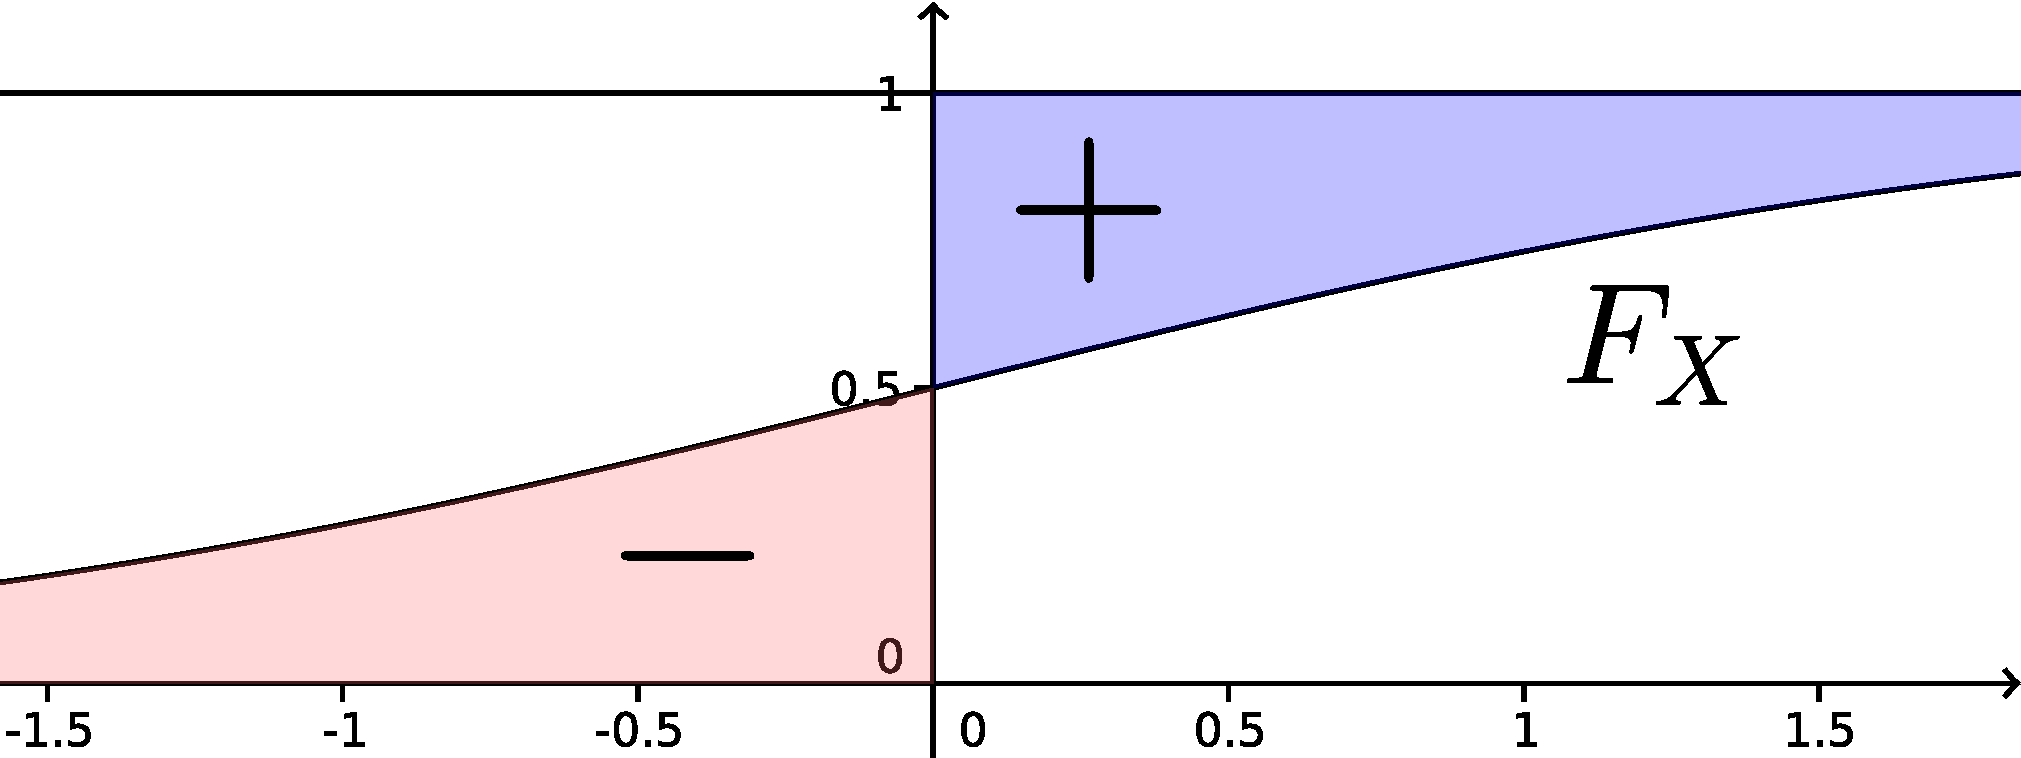
\includegraphics[width=7cm]{ex} & $$ \E X=\E X^+-\E X^-=\int\limits_{0}^{+\infty}(1-\FF_X(x))\dif x-\int\limits_{-\infty}^0 \FF_X(x)\dif x $$  
	\end{tabular} \newline
	za předpokladu konečnosti jednoho z integrálů.
\end{dusl}

\begin{theorem}[VPI - Věta o přenosu integrace]
	Nechť $\X\sim\PEX$ je náhodná veličina, $g:\R^n\to\R$ je borelovsky měřitelná. Pak $$ \int\limits_{\Omega}g\circ \X ~\dif \PP = \int\limits_{\R^n} g(\textbf{x})\dif(\underbrace{\PP\circ \X^{-1}}_{\PEX}) \text{ za předpokladu existence alespoň jednoho integrálu.}$$
	Navíc pokud $\X$ má $ASR_\lambda$ s $\fex~(\fex=\frac{\dif\PEX}{\dif\lambda})$, pak $$ \int\limits_{\Omega}g\circ \X \dif \PP = \int\limits_{\R} g(\textbf{x})\fex(\textbf{x})\dif\lambda,\text{ pokud }g(\X)\in\LL_1. $$ V případě, že $\X$ má diskrétní rozdělení, tzn. $\PP(\X=\textbf{x}_k)=p_k$, pak  $$ \int\limits_{\Omega}g\circ \X ~\dif \PP =\sum\limits_{k}g(\textbf{x}_k)p_k=\int\limits_{\R} g(\textbf{x})\fex(\textbf{x})\dif\mu_c\text{,~~ kde }\mu_c\{ \textbf{x}_k \}=1~~~\forall k \in\N.$$
	\begin{proof}
		\begin{enumerate}
			\item Nejprve dokážeme pro $g(\textbf{x})=\mathbb{I}_B(\textbf{x})$, $B\in\Bb$. 
			\[
			\begin{split}
			\E \left[ \mathbb{I}_B(\X) \right]&=\int\limits_{\Omega}\underbrace{\mathbb{I}_B(\X)}_{\neq 0,\X(\omega)\in B}\dif \PP=\int\limits_{\X^{-1}(B)} 1 \dif \PP= \PP\br{\X^{-1}(B)}=\PEX(B)=\int\limits_{B}1\dif\PEX=\\ &=\int\limits_{\R^n}\underbrace{\mathbb{I}_B(\textbf{x})}_{g(\textbf{x})}\dif(\PP\circ \X^{-1})
			\end{split}
			\]
			\item $g(\textbf{x})=\sum\limits_{j=1}^n b_j \mathbb{I}_{B_j}(\textbf{x})$ $$ \E \Bigl[ \sum\limits_{j=1}^n b_j \mathbb{I}_{B_j}(\X) \Bigr]=\sum\limits_{j=1}^n b_j \E \left[ \mathbb{I}_{B_j}(\X) \right]=\text{viz 1)} $$
			\item $g\geq 0$ libovolná $~\Rightarrow~ \exists h_n(\textbf{x})\nearrow g$, kde  $h_n$ je simple function.
			$$~\Rightarrow~ \E [g(\X)]=\E \Bigl[ \lim\limits_{ n\to +\infty} h_n(\X) \Bigr]\equal{\text{MCT}}\lim\limits_{ n\to +\infty} \E h_n(\X)=\text{ viz 2)}$$ 
			\item $g$ libovolná $~\Rightarrow~ g=g^+-g^- ~\Rightarrow~ \E [g(\X)]=\E g^+(\X)-\E g^-(\X)=$ viz 3)
		\end{enumerate}
	Pro diskrétní rozdělení použijeme Radon-Nikodymovu větu a pokračujeme analogicky.
	\end{proof}
\end{theorem}
\begin{example}
	\[
	\E Y=\int\limits_{\Omega}Y\dif \PP=\begin{cases}
	\int\limits_{\Omega}g\circ \X~\dif \PP=\int\limits_{\Omega}g\dif\PEX=\int\limits_{\Omega}g\frac{\dif\PEX}{\dif\lambda}\dif\lambda=\int\limits_{\Omega}g\fex \dif\lambda\equal{\lambda=\lambda_c}\sum\limits_{k}g(\textbf{x}_k)\fex(\textbf{x}_k)=\sum\limits_{k}g(\textbf{x}_k)p_k \\
	\int\limits_{\R}y\dif \PP^Y
	\end{cases}
	\]
	kde $\lambda_c$ je čítací míra definovaná pro izolované body jako $\lambda_c(\{\textbf{x}_k\})=1~~~\forall k\in\N$.
\end{example}
\begin{remark}
	$\int\limits_{\Omega}g\dif\PEX\equal{\text{ozn.}}\int\limits_{\Omega}g\dif\FEX$ (Lebesgue-Stieltjes integrals)
\end{remark}
\begin{theorem}
	Nechť $\posl$ je posloupnost nezávislých náhodných veličin na $\prostor$, \newline $X_j\in\LL_1$. Pak \[
	\E \Bigl[\underbrace{\prod\limits_{j=1}^n X_j}_{Y=g(\X)}\Bigr] =\prod\limits_{j=1}^n \E X_j~~~\forall n\in\N.
	\]
	\begin{proof}
		$$ \E Y\equal{\text{VPI}}\int\limits_{\R^n}\prod\limits_{j=1}^n x_j \dif\PEX \equal{\text{id.}}\int\limits_{\R^n}\prod\limits_{j=1}^nx_j\dif(\otimes \PP^{X_j})\equal{T-F.V.}\prod\limits_{j=1}^n \int\limits_{\R}x_j\dif \PP^{X_j}=\prod\limits_{j=1}^n \int\limits_{\Omega}X_j\dif \PP=\prod\limits_{j=1}^n \E X_j $$
	\end{proof}
\end{theorem}

\begin{define}~
	\begin{enumerate}
	\item $\LL_2\prostor=\{ X$ náhodná veličina na $\prostor:\E (X^2)\equal{\text{ozn}}\E X^2<+\infty,X^2\in\LL_2 \}$
	\item $	\\L_2(\Omega,\Aa,\PP_n)=\LL_2/_\sim,\text{ kde }X\sim Y\Leftrightarrow X=Y~s.j.~\PP $
	\item $ \E (X\cdot Y)=\langle X,Y\rangle  $
	\item $ \left\|X\right\|_2=\sqrt{\langle X|X\rangle}=\sqrt{\E X^2} $
	\end{enumerate}
\end{define}
\begin{remark}~
	 \begin{enumerate}
	 	\item $$ \E (X\cdot Y)=\langle X,Y\rangle=\int\limits_{\Omega}X\cdot Y\dif \PP\equal{\text{VPI}}\int\limits_{\R^2}x\cdot y\dif \PP^{(X,Y)}\equal{\text{ASR}}\int\limits_{\R^2}x\cdot yf_{X,Y}(x,y)\dif\lambda  $$
	 	\item $$ \langle X,X \rangle=0\Leftrightarrow X=0~s.j.~\PP $$
	 	\item korektnost: $$ |X\cdot Y|\leq 2X^2+2Y^2 $$
	 	$$ |\E (X\cdot Y)|\leq \E |X\cdot Y|\leq 2\E X^2+2\E Y^2<+\infty~~\forall X,Y\in\LL_2 $$
	 \end{enumerate}
\end{remark}
\begin{theorem}[Schwarz]
	Nechť $X,Y\in\LL_2$. Pak $X\cdot Y\in\LL_1$ a platí, že $|\E (X\cdot Y)|\leq \left\|X\right\|_2 \cdot \left\|Y\right\|_2$, přičemž $|\E (X\cdot Y)|= \left\|X\right\|_2 \cdot \left\|Y\right\|_2\Leftrightarrow (\exists\alpha\neq0)(Y=\alpha X~s.j.~\PP)$ (což je ale např. u Diracovy míry pouze v jednom bodě).
\end{theorem}
\begin{dusl}
	Prostor $ (\L_2, \left\|~\right\|_2) $ je úplný lineární normovaný prostor se skalárním součinem (Hilbertův).
\end{dusl}
\begin{theorem}
	$ \LL_2 \prostor\subset\LL_1\prostor$
	\begin{proof}
		$X\in\LL_2,~\LL_2\ni Y=1~s.j.~\PP$. Potom ze Schwarze plyne:
		$$ |\E (X\cdot Y)|=|\E X|\leq \sqrt{\E X^2\cdot \E 1^2}\leq \sqrt{\E X^2} $$
	\end{proof}
\end{theorem}
\begin{define}
	Mějme $ X\in\LL_2 $. Potom definujeme \textbf{rozptyl náhodné veličiny X} jako $$\D X(=\mathop{\mathrm{Var}} X):=\E (X-\E X)^2=\E (X^2-2X\cdot \E X+(\E X)^2)=\E X^2-(\E X)^2 \geq 0.$$
	Dále definujeme \textbf{směrodatnou odchylku} jako $\sigma(X):=\sqrt{\D X} $ a \textbf{standardizovanou náhodnou veličinu} jako $Y=\frac{X-\E X}{\sqrt{\D X}}$. ($\E Y=0,\D Y=1$)
\end{define}
\begin{remark}
	$$\E (b)=\int\limits_{\Omega}b \dif \PP=b\PP(\Omega)=b, ~~~  \forall b\in\R$$
\end{remark}
\begin{theorem}~\newline
	$ X\in\LL_2~\Rightarrow~ \D (\alpha X+\beta)=\E \left[ (\alpha X+\beta)-\E (\alpha X+\beta) \right]^2=\E \left[ \alpha(X-\E X) \right]^2=\alpha^2 \D X $
\end{theorem}
\begin{dusl}
	$ \D (\beta)=0 $, $ X=\beta~s.j.~\PP~\Rightarrow~ \D X=\E \left(0_{s.j.}^2\right)=0 $
\end{dusl}
\begin{define}
	Nechť $X,Y\in\LL_2\prostor$. Definujeme \textbf{kovarianci} jako \[
	\Cov(X,Y)=\E \left[ (X-\E X)(Y-\E Y) \right]=\E (X\cdot Y-X\E Y-Y\E X+\E X\cdot \E Y)=\E (X\cdot Y)-\E X\cdot \E Y
	\]
\end{define}
\begin{theorem}
	Pro kovarianci platí, že 
	\begin{enumerate}
		\item $ \Cov(X,X)=\D X\geq 0 $
		\item je symetrická
		\item $X,Y$ nezávislé $~\Rightarrow~ \Cov(X,Y)=0$ (definujeme $X,Y$ nekorelované)
		\item obměna 3): $\Cov(X,Y)\neq 0~\Rightarrow~ X$ a $Y$ nejsou nezávislé
	\end{enumerate}
	\begin{proof}
		\begin{enumerate}[3.]
			\item $\Cov(X,Y)=\E (X\cdot Y)-\E X\cdot \E Y=0$
		\end{enumerate}
	\end{proof}
\end{theorem}
\begin{example}	
	Nechť $X$ je náhodná veličina se symetrickým rozdělením okolo 0 \newline ($ X\sim \FF_X \Leftrightarrow -X\sim \FF_X $). Pak platí, že
	\begin{enumerate}
		\item $ Y=X^2 ~\Rightarrow~ \Cov(X,Y)=\Cov(X,X^2)=\underbrace{\E (X^3)}_{=0}-\underbrace{\E X}_{=0}\cdot \E X^2=0, $ protože \newline $\E X=\int\limits_{\Omega}x\dif \PP^X \equal{\text{ASR}}\int\limits_{-\infty}^{+\infty}xf_X(x)\dif x=0. $\newline
		$\Cov(X,Y)=0$, ale $X,X^2$ jsou závislé (ASR). Opačná implikace v 3) tedy neplatí. 
		\item $Y=X^3 ~\Rightarrow~ \Cov(X,X^3)=\E (X^4)-\E X\cdot \E X^3=\E (X^4)>0 $ pro nedegenerovanou veličinu.
	\end{enumerate}
	Celkově jsme tedy dospěli k závěru, že $\Cov(X,Y)$ není mírou závislosti/nezávislosti.
	
\end{example}
\begin{theorem}\label{Decko}
	Mějme nezávislé náhodné veličiny $(X_j)_{j=1}^n\in\LL_2$. Pak \[
	\D \left( \sum\limits_{j=1}^n X_j \right)=\sum\limits_{j=1}^n \D X_j.
	\] 
	\begin{proof}
		\[
		\begin{split}
		 \D \left( \sum\limits_{j=1}^n X_j \right)&=\E  \left( \sum\limits_{j=1}^n X_j - \E \sum\limits_{j=1}^n X_j \right)^2=\E \left( \sum\limits_{j=1}^n (X_j-\E X_j) \right)^2=\\ &=\E \left[ \sum\limits_{j=1}^n (X_j-\E X_j)^2 + \sum\limits_{i\neq j}(X_i-\E X_i)(X_j-\E X_j) \right]=\\ &=\left[ \sum\limits_{j=1}^n \E (X_j-\E X_j)^2 + \sum\limits_{i\neq j}\underbrace{\E \left[(X_i-\E X_i)(X_j-\E X_j)\right]}_{\Cov(X_i,X_j)=0~pro~i.d.} \right]=\sum\limits_{j=1}^n \D (X_j)+\sum\limits_{i\neq j}\Cov(X_i,X_j) 
		\end{split}
		\]
	\end{proof}
\end{theorem}
\begin{theorem}[Čebyševova nerovnost]
	Buď $X\in\LL_2$. Pak $(\forall \epsilon>0)\Bigl(\PP(|X-\E X|\geq \epsilon)\leq \frac{\D X}{\epsilon^2}\Bigr)$.
	\begin{proof}
		Markovova nerovnost: $ Y\in\LL_1~\Rightarrow~(\forall\epsilon>0)\left(\PP(|Y|\geq \epsilon)\leq \frac{\E |Y|}{\epsilon}\right) $ a dosadíme\newline $Y=(X-\E X)^2$, neboť víme, že $X \in \LL_2  \Rightarrow (X-\E X)^2\in \LL_1$. Potom $\forall \epsilon>0$ platí, že
		\[
		\begin{split}
		\PP(|(X-\E X)^2|\geq \epsilon^2)&\leq \frac{\E (X-\E X)^2}{\epsilon^2} \\ \PP(|X-\E X|\geq \epsilon)&\leq \frac{\D X}{\epsilon^2} 
		\end{split}
		\] 
	\end{proof}
\end{theorem}

\begin{define}
	Mějme náhodné veličiny $X,Y$, kde $\D X>0,~\D Y>0$ (nedegenerované). Definujeme \textbf{korelační koeficient} $$\rho(X,Y)=\rho_{XY}=\frac{\Cov(X,Y)}{\sqrt{\D X}\sqrt{\D Y}}.$$ 
\end{define}
\begin{theorem}
	Mějme náhodné veličiny $X,Y\in\LL_2$, kde $\D X>0,~\D Y>0$ (nedegenerované). Pak $ |\rho(X,Y)|\leq 1 $ a platí, že $$ \rho = \pm 1 \Leftrightarrow \exists \beta\gtrless 0\text{ tak, že }Y-\E Y=\beta(X-\E X) ~s.j.~\PP$$
	\begin{proof}
		$$ |\rho_{XY}|=\frac{|\E \left[ (X-\E X)(Y-\E Y) \right]|}{\sqrt{\E (X-\E X)^2}\sqrt{\E (Y-\E Y)^2}}=\frac{|\langle X-\E X,Y-\E Y\rangle_{\L_2} |}{\left\| X-\E X \right\|_{\L_2}\cdot \left\| Y-\E Y \right\|_{\L_2}}\leq 1\text{ (Schwarz)}, $$
		kde $|\rho_{XY}|=1\Leftrightarrow(\exists\beta\in\R\setminus\{0\})\left( Y-\E Y\equal{s.j.}\beta(X-\E X) \right)  $, tedy $$ \rho_{XY}=\frac{\E \left[ (X-\E X)(\beta(X-\E X)) \right]}{\sqrt{\E (X-\E X)^2}\sqrt{\E (\beta(X-\E X))^2}}=\frac{\beta\cdot \D X}{|\beta|\cdot \D X}=\pm 1 $$
	\end{proof}
\end{theorem}
\begin{define}
	Mějme $\X=(X_1,...,X_n)$, $X_j\in\LL_2$. Pak definujeme \textbf{kovarianční matici} vztahem
	\[
	\C(\X):=\left( \Cov(X_i,X_j) \right)_{i,j=1}^{+\infty}.
	\]
\end{define}
\begin{theorem}
	Nechť $\C(\X)$ je symetrická, PSD (pozitivně semidefinitní) a $\diag(\C)=(\D X_1,...,\D X_n)$. Pak pro $Y:=\sum\limits_{j=1}^n\alpha_jX_j$ platí, že $0\leq \boldsymbol\alpha\C\boldsymbol\alpha^T$.
	\begin{proof}
		\[
		\begin{split}
		0&\leq \D Y=\E \left( \sum\limits_{j=1}^n\alpha_jX_j-\E \Bigl( \sum\limits_{j=1}^n\alpha_jX_j \Bigr) \right)^2=\E \left( \sum\limits_{j=1}^n\alpha_j(X_j-\E X_j) \right)^2= \\ 
		&=\E \left( \sum\limits_{i=1}^n\sum\limits_{j=1}^n\alpha_j(X_j-\E X_j)(X_i-\E X_i) \alpha_i\right)= \sum\limits_{i=1}^n\sum\limits_{j=1}^n\alpha_j\E \Bigl((X_j-\E X_j)(X_i-\E X_i) \Bigr)\alpha_i= \\ 
		&=\sum\limits_{i=1}^n\sum\limits_{j=1}^n\alpha_j\Cov(X_i,X_j)\alpha_i=\boldsymbol\alpha\C\boldsymbol\alpha^T
		\end{split}
		\]
	\end{proof}
\end{theorem}
\begin{define}
	Definujeme 
	\begin{enumerate}
		\item $R(\X)=(\rho(X_i,X_j))_{i,j=1}^n$ jako \textbf{korelační matici}, kde $\diag\br{R(\X)}=\mathbb{I}$
		\item $\LL_{p\geq 1}=\{ X\text{ náhodná veličina na }\prostor: |X|^p\in\LL_1 \}$
		\item $\L_p=\LL_p/_\sim$ kde $X\sim Y \Leftrightarrow X=Y~s.j.~\PP$  
		\item pro náhodnou veličinu $X\in\LL_p$ definujeme funkci $\left\| X \right\|_p=\sqrt[p]{\E |X|^p}$
	\end{enumerate}

\end{define}
\begin{theorem}[Hölderova nerovnost]
	Nechť $X\in\LL_{p\geq 1}$ a $Y\in\LL_{q\geq 1}$ tak, že $\frac{1}{p}+\frac{1}{q}=1$. Pak $X\cdot Y \in\LL_1$ a platí vztah 
	$$ |\E (X\cdot Y)|\leq \E |X\cdot Y|\leq \left\|X\right\|_p\cdot \left\|Y\right\|_q  $$
	\begin{proof}
			Youngova nerovnost: $ c,d\geq 0~\Rightarrow~ c^{1/p}d^{1/q}\leq \frac{1}{p}c+\frac{1}{q}d $, kde $\frac{1}{p}+\frac{1}{q}=1$. Zbytek viz FA.
		
	\end{proof}
\end{theorem}
\begin{remark}
	Pro $p=q=2$ tuto nerovnost názýváme Schwarzovou.
\end{remark}
\begin{dusl}
	$\left\| X\right\|_p$ je pseudonorma na $\LL_{p\geq 1}$ a norma na $\L_p$.
\end{dusl}
\begin{theorem}
	Nechť $1\leq p\leq q< +\infty$. Pak $\LL_q\prostor\subset \LL_p\prostor$. (platí jen pro konečnou míru)
	\begin{proof}~
		$$ \left. \begin{array}{l}
	|X| \leq 1 ~\Rightarrow~ |X|^p \leq ~~1~~  \leq 1+|X|^q \\
	|X| \geq 1 ~\Rightarrow~ |X|^p \leq |X|^q  \leq 1+|X|^q 
		\end{array}  \right\}\Rightarrow |X|^p \leq 1+|X|^q  $$
		$$ \E |X|^p\leq \E (1)+ \E |X|^q=1+ \E |X|^q $$
	\end{proof}
\end{theorem}
\begin{define}
	Definujeme $\mu'_k(X)=\mu'_k=\E (X^k)$ za předpokladu, že $\E (X^k)$ existuje, $k\in\N$, a nazýváme ho \textbf{obecný k-tý moment} náhodné veličiny $X$. Definujeme dále \newline
	$ \mu_k(X)=\mu_k=\E \left[ (X-\E X)^k \right] $ jako \textbf{centrální k-tý moment} náhodné veličiny $X$ za předpokladu existence pravé strany, $k\in\N$.
	\begin{enumerate}
		\item $\mu'_1=\E X$, $\mu_1=0$
		\item $\mu_2=\D X$
		\item $\mu_3(U)=\mu_3\left( \frac{X}{\sigma(X)} \right)=\frac{\mu_3(X)}{[\sigma(X)]^3}$ nazýváme \textbf{šikmost rozdělení} náhodné veličiny X.\newline $\mu_3(U)=0~\Rightarrow~$ X má symetrické rozdělení okolo $\E X$.
		\item $\mu_4(U)=\mu_4\left( \frac{X}{\sigma(X)} \right)=\frac{\mu_4(X)}{[\sigma(X)]^4}$ nazýváme \textbf{špičatost rozdělení} náhodné veličiny X.\newline
		$\mu_4(U)=3$ pro libovolné $X\sim N(\mu,\sigma^2)$.
		\item $\mu_e:=\mu_4(U)-3$ nazveme \textbf{koeficient špičatosti}.
	\end{enumerate}
\end{define}
\begin{define}
	Definujeme $\LL_{\infty}:=\{ X\text{ náhodná veličina na }\prostor: X~s.j.~\PP\text{ omezená} \}$. Definujeme dále $\left\|X\right\|_{\infty}=\mathop{\mathrm{ess~sup}} X$ jako nejmenší konstantu $c$, pro kterou platí $|X|<c~~s.j.~\PP$.
\end{define}

\begin{theorem}
	Platí, že $\LL_{\infty}\subset \LL_{p\geq 1}$ a $\left\|~\right\|_{\infty}=\lim\limits_{ p\to +\infty}\left\|~\right\|_p$.
\end{theorem}
\section{Charakteristické funkce náhodných veličin}
\begin{define}
	Mějme $\X$ náhodnou veličinu na $\prostor$. Definujeme \textbf{charakteristickou funkci} náhodné veličiny $\X$~~ $\lphi_\X:\R^n\to\C $ vztahem $$\lphi_\X(\textbf{t}):= \E \underbrace{\bigl( \me^{\mi\textbf{t}\cdot \X} \bigr)}_{Y:\Omega\to \C}=\int\limits_{\Omega} \me^{\mi\textbf{t}\X}\dif \PP\equal{\text{VPI}}\underbrace{\int\limits_{\R^n}\me^{\mi\textbf{t}\textbf{x}}\dif\PEX}_{\mathfrak{F}(\PEX)}\equal{\text{ASR}}\underbrace{\int\limits_{\R^n}\me^{\mi\textbf{t}\textbf{x}}\fex(\textbf{x})\dif\lambda}_{\mathfrak{F}(\fex)}\equal{\lambda\text{ čítací}}\sum\limits_{k}\me^{\mi\textbf{t}x_k}\underbrace{\fex(x_k)}_{p_k},$$ kde $\mathfrak{F}$ je Fourierova transformace.
\end{define}
\begin{remark}~
	\begin{enumerate}
		\item Korektnost definice: Nechť $Z:\Omega\to\C$ je náhodná veličina $Z=X+ \mi  Y$. Potom 
		$$ \E Z=\E X+ \mi  \E Y,~~~\FF_Z=\FF_{(X,Y)}. $$
		\item Řekneme, že $Z\in\LL_1$ (ve smyslu $\C$) znamená, že $X,Y\in\LL_1$. 
		\item Tonelli-Fubiniho věta v $\C$ platí, tedy
		\[
		\begin{split}
		&\int\limits_{\Omega_1\times\Omega_2} Z(\omega_1,\omega_2)\dif \PP=\int\limits_{\Omega_1\times\Omega_2}\left( X(\omega_1,\omega_2)+ \mi  Y(\omega_1,\omega_2) \right)\dif \PP_1\otimes \dif \PP_2\equal{\text{F.V.}} \\ 
		&=\int\limits_{\Omega_2}\Bigl( \int\limits_{\Omega_1} X\dif \PP_1 \Bigr)\dif \PP_2+\mi \int\limits_{\Omega_2}\Bigl( \int\limits_{\Omega_1} Y\dif \PP_1 \Bigr)\dif \PP_2=\int\limits_{\Omega_2} \Bigl( \int\limits_{\Omega_1}(X+\mi Y)\dif \PP_1 \Bigr)\dif \PP_2 
		\end{split}
		\] 
		\item VPI pro transformaci do $\C$: Mějme $\X,~\tilde{g}:\R^n\to\C$. Pak
		$$ Z=\tilde{g}(\X)~~~~\Rightarrow~~~~\E Z=\int\limits_{\Omega}Z\dif \PP=\int\limits_{\R^n}\tilde{g}(\textbf{x})\dif\PEX $$
		\begin{proof}
			 $\tilde{g}(\X)=\Re \tilde{g}(\X)= \mi  \Im \tilde{g}(\X)~\Rightarrow~$
			\[
			\begin{split}
			\int\limits_{\Omega}\tilde{g}(\X)\dif \PP&=\int\limits_{\Omega} \Re \tilde{g}(\X)\dif \PP +  \mi  \int\limits_{\Omega}\Im\tilde{g}(\X)\dif \PP\equal{VPI~v~\R^n} \\
			&= \int\limits_{\R^n}\Re\tilde{g}(\textbf{x})\dif\PEX+ \mi  \int\limits_{\R^n}\Im\tilde{g}(\textbf{x})\dif\PEX=\int\limits_{\R^n}\tilde{g}(\textbf{x})\dif\PEX
			\end{split}
			\] 
		\end{proof}
	\end{enumerate}
\end{remark}

\begin{theorem} Mějme $\prostor$ s konečnou mírou. Potom pro $\lphi_\X$ platí: \begin{enumerate}
		\item vždy existuje,
		\item je omezená, $|\lphi_\X|\leq 1$,
		\item $\lphi_\X(\textbf{0})=1$,
		\item je spojitá.
		\item  Nechť dále $\X\in\LL_k$ po složkách. Pak $\lphi_\X\in\mathcal{C}^{k}$ a platí 
		$$ \frac{\partial \lphi_\X}{\partial t_{j_1}...\partial t_{j_k}}(\textbf{0})=\mi^k ~\E (X_{j_1}X_{j_2}...X_{j_k}). $$
	\end{enumerate}
	\begin{proof}~
		\begin{enumerate}[	a)]
			\item Existence: $\exists \lphi_\X(\textbf{t})=\E \left( \me^{ \mi  \textbf{t}\X} \right)=\E \bigl( \cos(\textbf{t}\cdot \X)+ \mi  \sin(\textbf{t}\cdot \X) \bigr)=\E \bigl(\cos(\textbf{t}\cdot \X)\bigr)+ \mi  \E \bigl(\sin(\textbf{t}\cdot \X)\bigr)$,
			kde $\cos(\textbf{t}\cdot \X)$ a $\sin(\textbf{t}\cdot \X)$ existují a jsou konečné.
			\item Omezenost: $|\lphi_\X(\textbf{t})|=\left| \E \left( \me^{ \mi  \textbf{t}\X} \right) \right|\leq \E \left| \me^{ \mi \textbf{t}\X} \right|=\E 1=1$
			\item $\lphi_\X(\textbf{0})=\E \left( \me^{ \mi  \textbf{0}\X} \right)=\E 1=1$
			\item Spojitost: $$\textbf{t}_n\to\textbf{t}_0:~~~\lim\limits_{ n\to +\infty}\lphi_\X(\textbf{t}_n)=\lim\limits_{ n\to +\infty}\E \parunderbrace{\left( \me^{\mi \textbf{t}_n\X}\right)}{\text{$\left| \me^{\mi \textbf{t}_n\X}\right|\leq 1\in\LL_1$} } \equal{\text{LDCT}}\E \left( \lim\limits_{ n\to +\infty}\me^{\mi \textbf{t}_n\X} \right)=\E \left( \me^{ \mi \textbf{t}_0\X} \right)=\lphi_\X(\textbf{t}_0)$$
			\item Nechť $\posl\in\LL_k$.
				$k=1:$
				$$\frac{\partial \lphi_\X}{\partial t_j}(\textbf{t})=\frac{\partial}{\partial t_j}\E \left( \me^{\mi \textbf{t}\X} \right)=\E \left( \frac{\partial}{\partial t_j}\me^{\mi \textbf{t}\X} \right)\equal{*}\E  \left(\mi  X_j\me^{\mi\textbf{t}\X}\right)  $$
				$(*)$ Použijeme vztah
				$$ \frac{\partial}{\partial t}\me^{\mi  t X}=\frac{\partial}{\partial t}\bigl(\cos(tX)+\mi \sin(tX)\bigr)=-X\sin(tX)+\mi  X\cos(tX)=\mi  X\bigl(\cos(tX)+\mi \sin(tX)\bigr)=\mi  X\me^{\mi  tX}. $$
				Z toho plyne, že $\frac{\partial}{\partial t_j}\lphi_\X(\textbf{0})=\mi  \E X_j$. 
				Spojitost $\frac{\partial}{\partial t_j}\lphi_\X$: $\textbf{t}_n\to\textbf{t}_0$:
				$$ \lim\limits_{ n\to +\infty}\frac{\partial \lphi_\X}{\partial t_j}(\textbf{t}_n)=\lim\limits_{ n\to +\infty}\E \left(\smash[b]{ \parunderbrace{ \mi  X_j\me^{\mi  \textbf{t}_n\X}}{\text{$\left| \mi  X_j\me^{\mi  \textbf{t}_n\X} \right|\leq |X_j|\in\LL_1$}}} \right)=\E \left( \mi  X_j \me^{\mi  \textbf{t}_0\X} \right)=\frac{\partial \lphi_\X}{\partial t_j}(\textbf{t}_0) $$
				$k=2$:
				$$ \frac{\partial^2 \lphi_\X}{\partial t_l\partial t_j}(\textbf{t})=\frac{\partial}{\partial t_l}\E \left( \mi  X_j \me^{\mi \textbf{t}\X} \right)=\E \left( \mi  X_j \mi  X_l \me^{\mi \textbf{t}\X} \right)=\mi ^2\E ( X_jX_l\me^{\mi  \textbf{t}\X}), $$
				kde $\left| X_jX_l\me^{\mi  \textbf{t}\X} \right|\leq|X_jX_l|\in\LL_1$, protože $X_j,X_l\in\LL_2. $ Z toho vyplývá, že 
				$$ \frac{\partial^2 \lphi_\X}{\partial t_l\partial t_j}(\textbf{0})=\mi ^2\E \left(  X_jX_l\right). $$
				Spojitost ověříme obdobně, jako pro $k=1$. 
			
			Potom stačí provést indukční krok $k\to k+1$. (ponecháno čtenáři)
		\end{enumerate}
	\end{proof}
\end{theorem}

\begin{dusl} Platí, že
	 \[
	\begin{split}
	(X,Y)\in\LL_{r+s}~~~&\Rightarrow~~~\E \left( X^rY^s \right)=(-1)^{r+s}~\mi ^{r+s}~\frac{\partial \lphi_\X}{\partial t_1^r \partial t_2^s}(0,0) \\
	X\in\LL_r,~s=0~~~&\Rightarrow~~~\mu'_r(X)=\E \left( X^r \right)=(-1)^r~\mi^r ~\frac{\partial \lphi_\X}{\partial t_{(1)}^r}(0)
	\end{split}
	\]
	Speciálně pak $ \D X= \E \left( X^2 \right)-(\E X)^2=-\frac{\partial^2 \lphi_\X}{\partial t^2}(0)-\left( -\mi  \frac{\partial \lphi_\X}{\partial t}(0) \right)^2=-\frac{\partial^2 \lphi_\X}{\partial t^2}(0)+\left(  \frac{\partial \lphi_\X}{\partial t}(0) \right)^2 $.
\end{dusl}
\begin{define}
	Mějme náhodnou veličinu $ \X\sim\PEX$. Pak definujeme \textbf{momentovou vytvářející funkci} (MGF) vztahem \[
	\mex(\textbf{t})=\E \left( \me^{\textbf{t}\X} \right)\equal{\text{VPI}}\underbrace{\int\limits_{\R^n}\me^{\textbf{tx}}\dif\PEX}_{\LL(\PEX)}\equal{\PEX\ll\lambda}\underbrace{\int\limits_{\R^n}\me^{\textbf{tx}}\fex(\textbf{x})\dif\textbf{x}}_{\LL(\fex)}
	\]
	Vlastnosti $\lphi_\X$ aplikovatelné i na $\mex$: \begin{enumerate}[	a)]
		\item Ne (existence)
		\item Ne (omezenost)
		\item Ano ($\mex(\textbf{0})=\E 1=1$)
		\item Ano (spojitost)
		\item Ano. Nechť $\X\in\LL_k$ po složkách. Pak $\mex\in\mathcal{C}^{k}$ a platí 
		$$ \frac{\partial \mex}{\partial t_{j_1}...\partial t_{j_k}}(\textbf{0})= \E (X_{j_1}X_{j_2}...X_{j_k}). $$
	\end{enumerate}
\end{define}
\begin{theorem}
	Mějme náhodnou veličinu $X:\Omega\to\R^1$. Nechť $\m_X(t)$ existuje na nějakém okolí $H_{t=0}$. Pak \[
	\lphi_X(t)=\m_X(\mi  t)=\E \left.\left( \me^{\mu X} \right)\right|_{\mu=\mi  t}=\E \left( \me^{\mi  tX} \right)~~~\forall t\in\R
	\]
	\begin{proof}
		Funguje dle věty o jednoznačnosti prodloužení analytické funkce z $H_0$ na $\C$.
	\end{proof}
\end{theorem}
\begin{example}
	Nechť $X\sim N(\mu,\sigma^2)$. Pak \[
	\lphi_X(t)=\me^{\mi t\mu-\frac{t^2\sigma^2}{2}}
	\]
	Možnosti důkazu:
	\begin{enumerate}
		\item $$\lphi_X(t)=\E \left(\me^{\mi  tX} \right)\equal{\text{VPI}}\int\limits_{\R} \cos(tx)\dif \PP^X+\mi  \int\limits_{\R}  \sin(tx)\dif \PP^X\equal{\text{ASR}}\int\limits_{\R} \cos(tx)f_X(x)\dif x+\mi  \int\limits_{\R} \sin(tx)f_X(x)\dif x$$
		\item Reziduová věta 
		\item Pokud $Y\sim N(0,1)$, pak $$\m_Y(t)=\E \left( \me^{tY} \right)=\int\limits_{\R}\me^{ty}\frac{1}{\sqrt{2\pi}}\me^{-\frac{y^2}{2}}\dif y= \frac{1}{\sqrt{2\pi}}\me^{\frac{t^2}{2}}\int\limits_{\R}\me^{-\frac{1}{2}(y-t)^2}\dif y=\me^{\frac{t^2}{2}} ~~~\forall t\in\R$$ je analytická (existuje taylorův rozvoj). Pro $z\in\C$ definujeme $\widetilde{\m}_Y(z):=\me^{z^2/2}$,
		$$\widetilde{\m}_Y(\mi t)=\me^{-t^2/2}=\lphi_X(t).$$
	 $$ \E Y=-\mi \left.\left(\frac{\dif}{\dif t} \me^{-t^2/2} \right)\right|_{t=0}=\mi  t \left.\left(\me^{-t^2/2}\right)\right|_{t=0}=0 ~\Rightarrow~ \E X=\E (\sigma Y+\mu)=\sigma \E Y+\mu=\mu$$
		Pokud $X=\sigma Y + \mu $, pak $ X\sim N(\mu,\sigma^2)$.
		$$ \lphi_X(t)=\lphi_{\sigma Y + \mu}(t)=\E \left( \me^{\mi  t(\sigma Y+\mu)} \right)=\E \left( \me^{\mi (\sigma t)Y}\me^{\mi  t \mu} \right)=\me^{\mi  t \mu}\lphi_Y(\sigma t)=\me^{\mi  t \mu}\me^{-\frac{\sigma^2t^2}{2}} $$
	\end{enumerate}
\end{example}
\begin{remark}
	\begin{enumerate}
		\item 	$ \D Y=\E Y^2-(\E Y)^2=\m'_Y(0)=1 $
		\item $ \D X=\D (\mu+\sigma Y)=\D (\sigma Y)=\sigma^2 \D Y=\sigma^2 $
		\item $ \E X^4=\int\limits_{\Omega} X^4\dif \PP\equal{\text{VPI}}\int\limits_{\R}x^4 \dif \PP^X\equal{\text{ASR}}\int\limits_{\R} x^4 f_X(x)\dif\lambda $
	\end{enumerate}
\end{remark}
\begin{example}
	$X\sim Cauchy(0,1)$, tedy $f_X(x)=\frac{1}{\pi(1+x^2)}$, $\m_X(t)=\E \left( \me^{tX} \right)\equal{\text{VPI}}\int\limits_{-\infty}^{+\infty}\frac{\me^{tx}}{\pi(1+x^2)}\dif x$, který diverguje vyjma $t=0$, kde $\m_X(0)=1$. Musíme proto střední hodnotu vypočítat ručně:
	$ \E X=\int\limits_{-\infty}^{+\infty}x\frac{1}{\pi(1+x^2)}\dif x=+\infty $, přestože např. $\lphi_X(t)$ vždy existuje.
\end{example}
\begin{theorem}
	Nechť $(X_j)_{j=1}^n$ jsou náhodné veličiny na $\prostor$ s rozdělením $\PP^{X_j}$. Pokud $\posl$ jsou nezávislé, tak platí, že 
	$$ \lphi_{\sum_{1}^{n}X_j}(t)=\prod\limits_{j=1}^n \lphi_{X_j}(t)~~~\forall t\in\R. $$ 
	Pokud existuje $\m_{X_j}$, pak analogicky platí, že $\m_{\sum_{1}^{n}X_j}(t)=\prod\limits_{j=1}^{n}\m_{X_j}(t)$.
	\begin{proof} Označme $Y=\sum\limits_{j=1}^{n}X_j$. Pak
		\[
		\begin{split}
		\lphi_Y(t)&=\underbrace{\E \left( \me^{\mi tY} \right)}_{\int\limits_{\R}\me^{\mi ty}\dif \PP^Y}\equal{VPI~v~\C}\E \left( \me^{\mi t\sum_{1}^{n} X_j} \right)=\int\limits_{\R^n}\me^{\mi t\sum_{1}^nx_j}\dif\PEX \equal{\text{id}}\int\limits_{\R^n}\Bigl( \prod\limits_{j=1}^n \me^{\mi tx_j} \Bigr)\dif\Bigl( \bigotimes\limits_{j=1}^n \PP^{X_j} \Bigr)\equal{T-F.V.} \\
		&=\prod\limits_{j=1}^n\int\limits_{\R}\me^{\mi tx_j}\dif \PP^{X_j}\equal{VPI~v~\C}\prod\limits_{j=1}^n \E \left( \me^{\mi tX_j} \right)=\prod\limits_{j=1}^n \lphi_{X_j}(t),
		\end{split}
		\] 
		případně můžeme využít toho, že ~ $ \left( X\sim f_X,~Y\sim f_Y \text{ nezávislé}~\Rightarrow~ f_{X+Y}=f_X\ast f_Y \right) $.
	\end{proof}
\end{theorem}
\begin{example}
	(Reprodukční vlastnost $N$). 
	Nechť $X_j\sim N(\mu_j,\sigma_j^2)$ jsou nezávislé. Pak 
	$$ \sum\limits_{j=1}^n X_j\sim N\biggl( \sum\limits_{j=1}^n \mu_j,\sum\limits_{j=1}^n \sigma_j^2 \biggr). $$
	\begin{proof}
		\begin{enumerate}
			\item Trasformační věta pro hustoty.
			\item $$ \lphi_{\sum_{1}^{n}X_j}(t)=\prod\limits_{j=1}^n \lphi_{X_j}(t)=\prod\limits_{j=1}^n \left( \me^{\mi t \mu_j-\frac{t^2\sigma_j^2}{2}} \right)=\me^{\mi t\sum_{1}^n\mu_j-\frac{t^2}{2}\sum_{1}^n \sigma_j^2}=\me^{\mi t\tilde{\mu}-\frac{t^2}{2}\tilde{\sigma}^2}\sim N(\tilde{\mu},\tilde{\sigma}^2), $$
			kde $\tilde{\mu}:=\sum\limits_{j=1}^n \mu_j $~ a ~$\tilde{\sigma}^2:=\sum\limits_{j=1}^n \sigma_j^2$.
		\end{enumerate}
	\end{proof}
\end{example}
\begin{theorem}[Inverzní formule]
	Nechť $X:\Omega\to\R$ je náhodná veličina s $\FF_X$. Pro pro $\forall a,b\in\R$, kde $a<b$ jsou body spojitosti $\FF_X$ platí, že 
	\[
	\PP^X\bigl((a,b]\bigr)=\PP(a<X\leq b)=\FF_X(b)-\FF_X(a)=\frac{1}{2\pi}\lim\limits_{ c\to +\infty}\int\limits_{-c}^c\frac{\me^{-\mi at}-\me^{-\mi bt}}{\mi t}\lphi_X(t)\dif t.
	\]
\end{theorem}
\begin{dusl}
	Charakteristická funkce $\lphi_X$ jednoznačně určuje $\PP^X$. Pro libovolné $b\in\R$ pak platí, že $\FF_X$ je v b spojitá zprava.
\end{dusl}
\begin{theorem}
	Mějme náhodnou veličinu $X$ s $\lphi_X$. Nechť $\lphi_X\in \L_1(\R,\dif x)$. Pak $$\exists f_X(x)=\frac{1}{2\pi}\int\limits_{-\infty}^{+\infty}\me^{-\mi tx}\lphi_X(t)\dif t=\mathfrak{F}^{-1}(\lphi_X).~~~(f_X\text{ je nutně spojitá a omezená})$$
	\begin{proof}
		Mějme $a<b$ body spojitosti $\FF_X$.
		\[
		\begin{split}
		\int\limits_{a}^b f_X(x)\dif x&=\frac{1}{2\pi}\lim\limits_{ c\to +\infty}\int\limits_{-c}^c\Br{\lphi_X(t)\int\limits_{a}^b \me^{-\mi tx}\dif x}\dif t=\frac{1}{2\pi}\lim\limits_{ c\to +\infty}\int\limits_{-c}^c \lphi_X(t)\frac{\me^{-\mi ta}-\me^{-\mi tb}}{\mi t}\dif t= \\ &=\FF_X(b)-\FF_X(a)=\PP^X\br{(a,b]}
		\end{split}
		\] 
		Dále $f_X\geq 0$, protože $\forall a,b \in\R, ~a<b$ platí, že 
		$$\int\limits_{a}^b f_X(x)\dif x\geq 0,~~~~~\int\limits_{-\infty}^{+\infty}f_X(x)\dif x=\FF_X(+\infty)-\FF_X(-\infty)=1.$$
	\end{proof}
\end{theorem}
\begin{lemma}\label{lematko}
	Mějme $\X,\lphi_\X$ a nechť $\I\in\tau_{4,n}=\{ \bigtimes\limits_{j=1}^n (a_j,b_j]:a_j,b_j\in\R \}$. Pak $$ \PEX(\I)=\PP(\X\in \I)=\frac{1}{(2\pi)^n}\lim\limits_{ c\to +\infty}\int\limits_{-c}^c\prod\limits_{j=1}^n\left( \frac{\me^{-\mi at_j}-\me^{-\mi bt_j}}{\mi t_j} \right)\lphi_\X(\textbf{t})\dif\textbf{t}. $$
\end{lemma}
\begin{theorem}
	Nechť $\X$ je náhodná veličina do $\R^n$. Pak $\lphi_\X \leftrightarrow \PEX$.\begin{proof}
		Plyne z lemmatu \ref{lematko}.
	\end{proof}
\end{theorem}
\begin{theorem}
	Mějme $\X=(X_1,...,X_n)$ náhodnou veličinu do $\R^n$. Potom platí, že\newline $X_1,...,X_n$ jsou nezávislé $\Leftrightarrow \lphi_\X(\textbf{t})=\prod\limits_{j=1}^n \lphi_{X_j}(t_j)$, $\forall\textbf{t}\in\R^n$.
	\begin{proof}
		\begin{enumerate}[$~\Rightarrow~$:]
			\item \[
			\begin{split}
			\lphi_\X(\textbf{t})&=\E \br{\me^{\mi \textbf{t}\X}}=\E \left( \me^{\mi \sum_{1}^n t_jX_j} \right)=\E \Bigl( \prod\limits_{j=1}^n \me^{\mi t_jX_j} \Bigr)\equal{\text{VPI}~v~\C} \\ &= \int\limits_{\R^n} \Bigl( \prod\limits_{j=1}^n \me^{\mi t_jx_j} \Bigr)\underbrace{\dif\PEX}_{\dif \Br{\bigotimes\limits_{j=1}^n \PP^{X_j}}}\equal{\text{T-F.V.}~v~\C}\prod\limits_{j=1}^n \underbrace{\int\limits_{\R} \me^{\mi t_jx_j }\dif \PP^{X_j} }_{\lphi_{X_j}(t_j)}
			\end{split}
			\] 
		\end{enumerate}
		\begin{enumerate}[$\Leftarrow$:]
		\item \[
		\begin{split}
		L&=\lphi_\X(\textbf{t})=\int\limits_{\R^n}\me^{\mi \textbf{t}\textbf{x}}\dif\PEX=\mathfrak{F}(\PEX) \\
		\PP&=\prod\limits_{j=1}^n \lphi_{X_j}(t_j)=\prod\limits_{j=1}^n \Br{\int\limits_{\R}\me^{\mi t_jx_j}\dif \PP^{X_j}}\equal{\text{T-F.V.}~v~\C}\int\limits_{\R^n}\Br{ \prod\limits_{j=1}^n \me^{\mi t_jx_j}} \dif\Br{ \bigotimes\limits_{j=1}^n \PP^{X_j}}= \\ &=\int\limits_{\R^n}\me^{\mi \textbf{t}\textbf{x}}\dif\Br{\bigotimes\limits_{j=1}^n \PP^{X_j}} =\mathfrak{F} \Br{\bigotimes\limits_{j=1}^n \PP^{X_j}} \\
		L&=\PP \text{ plyne z předpokladu, tzn. } \mathfrak{F}(\PEX)=\mathfrak{F}\Bigl(\bigotimes\limits_{j=1}^n \PP^{X_j}\Bigr)
		\end{split}
		\] 
		Z jednoznačnosti potom $\PEX=\bigotimes\limits_{j=1}^n \PP^{X_j}$, z čehož plyne nezávislost $X_j$.
	\end{enumerate}
	\end{proof}
\end{theorem}